% Compile with: tectonic DiagrammaticReasoning.tex   (or xelatex/pdflatex twice)
\documentclass[11pt]{article}
\usepackage[T1]{fontenc}
\usepackage[utf8]{inputenc}
\usepackage{lmodern}
\usepackage[margin=2.4cm]{geometry}
\usepackage{amsmath,amssymb,amsthm}
\usepackage{mathtools}
\usepackage{tikz}
\usepackage{tikz-cd}
\usetikzlibrary{arrows.meta,calc,positioning,decorations.pathreplacing,decorations.markings,
  patterns,shapes.geometric,fit,backgrounds,intersections}
\usepackage{booktabs}
\usepackage{longtable}
\usepackage{caption}
\usepackage{float}
\usepackage{enumitem}
\usepackage[colorlinks=true,linkcolor=blue!50!black,urlcolor=blue!50!black,
  citecolor=blue!50!black]{hyperref}

\theoremstyle{definition}
\newtheorem{recipe}{Recipe}[section]
\theoremstyle{plain}
\newtheorem{claim}{Claim}[section]
\theoremstyle{remark}
\newtheorem{trap}{Trap}[section]

\newcommand{\dd}{\operatorname{d}}
\newcommand{\Met}{\mathbf{Met}}
\newcommand{\id}{\mathrm{id}}
\newcommand{\R}{\mathbb{R}}
\newcommand{\N}{\mathbb{N}}
\newcommand{\lean}[1]{\texttt{#1}}
\newcommand{\norm}[1]{\lVert #1\rVert}

\tikzset{
  box/.style   = {draw, thick, fill=white, minimum width=9mm, minimum height=7mm,
                  rounded corners=1pt},
  wire/.style  = {thick},
  dot/.style   = {circle, fill=black, inner sep=2.1pt},
  odot/.style  = {circle, draw, thick, fill=white, inner sep=2.1pt},
  vec/.style   = {-{Stealth[length=2.5mm]}, very thick},
  axis/.style  = {-{Stealth[length=2mm]}, gray!60!black},
}

\title{\bfseries Drawing the two overlaps\\[2mm]
\large Diagrammatic reasoning about the \emph{triangle inequality} and the \emph{inverse},
with a picture atlas for \emph{Kalkulus I} and \emph{Line\'aris algebra I}}
\author{}
\date{}

\begin{document}
\maketitle
\vspace{-10mm}

\begin{abstract}
\noindent
Two items occur in both the \emph{Kalkulus I} and the \emph{Line\'aris algebra I}
\emph{t\'argytematika}: the \textbf{triangle inequality} (``nevezetes
egyenl\H otlens\'egek'' / ``vektorok hossza, h\'aromsz\"og-egyenl\H otlens\'eg'') and the
\textbf{inverse with respect to composition} (``inverz f\"uggv\'eny, \"osszet\'etel'' /
``m\'atrixok inverze''). The companion Lean files show that in each case the two courses
state one thing: the triangle inequality \emph{is} composition in a category enriched
over $([0,\infty),\ge,+)$, and the inverse \emph{is} isomorphism in a category. This
document asks the complementary question: \emph{how do you draw that, and how far can a
drawing alone carry a proof?} We survey eight diagrammatic languages -- commutative
diagrams, string diagrams (``graphical linear algebra''), proofs without words,
number-line and $\varepsilon$-interval pictures, Cartesian graphs and the mirror $y=x$,
Euler/Venn and bag-and-arrow diagrams, order (Hasse) diagrams, and geometric optimisation
pictures. For each we state its marks, its legal moves and whether it is certified, and
then work through the exercises of \lean{kalkulus\_gyakorlo.pdf} that can be settled by
drawing. The last section is a playbook for a timed exam. Every mathematical claim
illustrated here is stated and proved in \lean{RequestProject/DiagramProofs.lean}; the
captions name the corresponding theorem.
\end{abstract}

\tableofcontents

% ==========================================================================
\section{What has to be true for a drawing to be a proof}
\label{sec:what}

A picture is a proof when it is a term of a formal language whose syntax happens to be
two-dimensional. Three separate things must be in place.

\begin{description}[leftmargin=2.2em,style=nextline]
\item[Syntax.] A fixed finite stock of marks (arrows, boxes, wires, dots, segments,
  shaded regions) and a rule saying which arrangements of marks are well formed. A doodle
  that is not well formed is not a statement at all, so it can be neither a proof nor a
  mistake -- it is noise.
\item[Legal moves.] A list of allowed transformations of one well-formed diagram into
  another: pasting two commuting cells, sliding a box along a wire, cutting a region and
  reassembling it, reflecting a graph in $y=x$.
\item[Soundness.] A theorem -- proved once, symbolically, \emph{outside} the picture
  language -- saying: if a diagram $D$ can be turned into $D'$ by legal moves, then the
  statement denoted by $D$ implies the statement denoted by $D'$.
\end{description}

The third point splits the languages below into two very different classes.

\begin{itemize}
\item \textbf{Certified languages.} Commutative diagrams and string diagrams come with a
  proved soundness, and often completeness, theorem. For string diagrams in a monoidal
  category, two diagrams are related by planar deformation exactly when the corresponding
  algebraic terms are equal (Joyal--Street). Here the drawing \emph{is} the term: you are
  not illustrating a proof, you are writing one.
\item \textbf{Heuristic languages.} A dissection picture, a number-line sketch or a
  Cartesian graph has no such theorem behind it. It proves something only relative to a
  small \emph{symbolic residue}: which configuration is generic, which case is missing,
  whether the curve really is monotone. In practice the residue is one or two lines.
\end{itemize}

\begin{center}
\small
\begin{tabular}{@{}llll@{}}
\toprule
Language & Marks & Legal move & Certified? \\
\midrule
Commutative diagrams   & objects, arrows        & pasting, filling & yes \\
String diagrams        & boxes, wires, spiders  & planar isotopy, rewriting & yes \\
Proofs without words   & regions, lengths       & dissection, superposition & no \\
Number line            & points, intervals      & translation, reflection & no \\
Cartesian graphs       & curves, lines          & reflection, transformation & no \\
Euler / bag-and-arrow  & blobs, dots, arrows    & containment, chaining & partly \\
Hasse / order          & nodes, upward edges    & path composition & yes \\
Geometric optimisation & figures, envelopes     & superposition & no \\
\bottomrule
\end{tabular}
\end{center}

\medskip
\noindent
Hence the rule of thumb we return to in Section~\ref{sec:exam}: \emph{use a certified
language when the statement is about composition or invertibility; use a heuristic
language when the statement is about a quantity, and write its symbolic residue on one
line next to the picture.}

% ==========================================================================
\section{Language A: commutative diagrams}
\label{sec:catdiag}

\paragraph{Marks.} Dots (objects) and arrows (morphisms); an arrow may be labelled.
\paragraph{Legal moves.} \emph{Pasting}: two commuting cells sharing an edge form a
commuting region. \emph{Filling}: if all inner cells commute, the outer boundary commutes.
\paragraph{Soundness.} Associativity and unitality of composition; this is a theorem, and
it is why the language is safe.

\subsection{The inverse, in four arrows}

``$g$ is inverse to $f$'' is by definition a statement about two triangles.

\begin{figure}[H]
\centering
\begin{tikzcd}[column sep=large,row sep=large]
X \arrow[r,"f"] \arrow[dr,"\id_X"'] & Y \arrow[d,"g"] \\
 & X
\end{tikzcd}
\qquad
\begin{tikzcd}[column sep=large,row sep=large]
Y \arrow[r,"g"] \arrow[dr,"\id_Y"'] & X \arrow[d,"f"] \\
 & Y
\end{tikzcd}
\qquad
\begin{tikzcd}[column sep=large,row sep=large]
Y \arrow[r,"g'"] \arrow[dr,"\id_Y"'] & X \arrow[d,"f"] \arrow[r,"g"] & Y \\
 & Y \arrow[ur,"g"'] &
\end{tikzcd}
\caption{Left and centre: the two triangles that say $g=f^{-1}$. Right: pasting the
left-inverse triangle of $g'$ onto the arrow $g$ shows $g'=g'\circ\id=g'\circ(f\circ g)
=(g'\circ f)\circ g=\id\circ g=g$. The inverse is unique -- drawn, not computed.
Certified in \lean{DiagramProofs.inverse\_unique} and, in an arbitrary category, in
\lean{SyllabusOverlap.inverse\_unique}.}
\label{fig:invunique}
\end{figure}

One picture covers both halves of the syllabus overlap:
\begin{itemize}\itemsep2pt
\item \emph{Kalkulus}, exercises 2.3--2.9 of \lean{kalkulus\_gyakorlo.pdf}: an answer
  $f^{-1}$ is right precisely when \emph{both} triangles close. Students routinely check
  only one; the diagram makes the omission visible.
\item \emph{Line\'aris algebra}: $MN=I$ with $\det M\neq 0$ forces $N=M^{-1}$ -- the same
  figure with $X=Y=\R^n$ and arrows the linear maps.
\end{itemize}

\subsection{The triangle inequality as composition (Lawvere)}

The triangle inequality looks like a statement about numbers, not a diagram. Lawvere's
observation is that it \emph{is} a composition law. Read a metric space as a category
whose objects are the points, whose hom-object from $x$ to $y$ is the number $\dd(x,y)$,
whose composition is $+$, and in which ``$\ge$'' is the direction of implication.

\begin{figure}[H]
\centering
\begin{tikzcd}[column sep=huge,row sep=large]
x \arrow[r,"\dd(x{,}y)"] \arrow[dr,"\dd(x{,}z)"'] & y \arrow[d,"\dd(y{,}z)"] \\
 & z
\end{tikzcd}
\qquad\raisebox{10mm}{$\rightsquigarrow$}\qquad
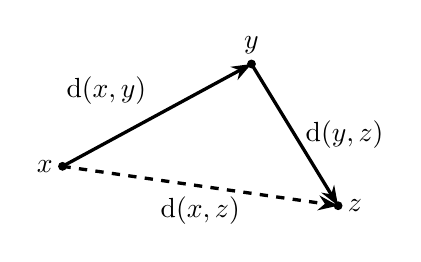
\begin{tikzpicture}[baseline=(current bounding box.center)]
  \coordinate (x) at (0,0);
  \coordinate (y) at (2.4,1.3);
  \coordinate (z) at (3.5,-0.5);
  \draw[vec] (x) -- node[above left]{$\dd(x,y)$} (y);
  \draw[vec] (y) -- node[right]{$\dd(y,z)$} (z);
  \draw[vec,dashed] (x) -- node[below]{$\dd(x,z)$} (z);
  \fill (x) circle (1.6pt) node[left]{$x$};
  \fill (y) circle (1.6pt) node[above]{$y$};
  \fill (z) circle (1.6pt) node[right]{$z$};
\end{tikzpicture}
\caption{The same statement twice. Left: the composite arrow $x\to z$ exists \emph{at
cost} $\dd(x,y)+\dd(y,z)$, while the hom-object $\dd(x,z)$ records the cheapest cost;
hence $\dd(x,z)\le\dd(x,y)+\dd(y,z)$. Right: the schoolbook triangle. Certified in
\lean{DiagramProofs.detour}.}
\label{fig:lawvere}
\end{figure}

Two things become visible in the categorical drawing that the schoolbook triangle hides.

\begin{figure}[H]
\centering
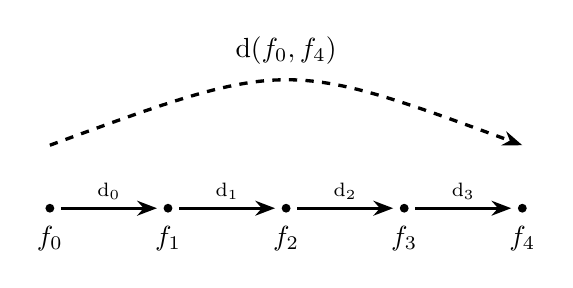
\begin{tikzpicture}[x=1cm,y=1cm]
  \foreach \i/\lab in {0/{f_0},1/{f_1},2/{f_2},3/{f_3},4/{f_4}}
    {\fill (1.5*\i,0) circle (1.6pt) node[below=3pt]{$\lab$};}
  \foreach \i in {0,1,2,3}
    {\draw[vec] (1.5*\i+0.14,0) -- (1.5*\i+1.36,0);}
  \draw[vec,dashed] (0,0.8) .. controls (3,1.9) .. (6,0.8);
  \node at (3,2.0) {$\dd(f_0,f_4)$};
  \node at (0.75,0.22) {$\scriptstyle \dd_0$};
  \node at (2.25,0.22) {$\scriptstyle \dd_1$};
  \node at (3.75,0.22) {$\scriptstyle \dd_2$};
  \node at (5.25,0.22) {$\scriptstyle \dd_3$};
\end{tikzpicture}
\caption{Composing a \emph{chain}: iterate the pasting move $n-1$ times to get
$\dd(f_0,f_n)\le\sum_{i<n}\dd(f_i,f_{i+1})$. With $f_k=\sum_{i<k}a_i$ in $\R$ this is
exercise 1.13 (generalised triangle inequality); with $f_k=\sum_{i<k}v_i$ in $\R^n$ it is
$\norm{\sum v_i}\le\sum\norm{v_i}$. One drawing, two courses. Certified in
\lean{TriangleOverlap.dist\_chain} and \lean{DiagramProofs.abs\_sum\_range\_le\_sum\_abs}.}
\label{fig:chain}
\end{figure}

\begin{figure}[H]
\centering
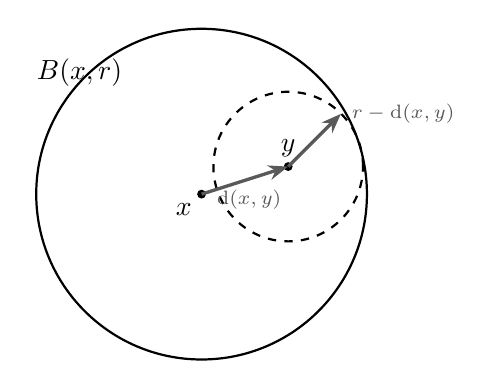
\begin{tikzpicture}[scale=1.0]
  \draw[thick] (0,0) circle (2.1);
  \node at (-1.55,1.55) {$B(x,r)$};
  \fill (0,0) circle (1.6pt) node[below left]{$x$};
  \coordinate (y) at (1.1,0.35);
  \draw[thick,dashed] (y) circle (0.95);
  \fill (y) circle (1.6pt) node[above]{$y$};
  \draw[vec,gray!70!black] (0,0) -- node[below,pos=0.55,font=\scriptsize]{$\dd(x,y)$} (y);
  \draw[vec,gray!70!black] (y) -- ++(0.67,0.67)
        node[right,font=\scriptsize]{$r-\dd(x,y)$};
\end{tikzpicture}
\caption{The triangle inequality drawn as an \emph{inclusion of discs}: if
$\dd(x,y)<r$ then $B\bigl(y,\,r-\dd(x,y)\bigr)\subseteq B(x,r)$. This is the picture
every ``open set'' and every limit argument in the course actually uses; drawing the two
nested circles is equivalent to writing the inequality. Certified in
\lean{DiagramProofs.ball\_subset\_ball\_of\_mem}.}
\label{fig:balls}
\end{figure}

\begin{recipe}[Draw an estimate as an arrow]
Whenever the quantity you must bound is the ``cost of getting from $A$ to $B$'', draw $A$
and $B$ as dots and every estimate you already have as a labelled arrow. Chaining arrows
adds costs; the bound you want is the cheapest path. Every $\varepsilon/3$ argument in
\emph{Kalkulus I} is this picture with three arrows:
\[
|f(x)-L|\;\le\;\underbrace{|f(x)-f_n(x)|}_{\varepsilon/3}
+\underbrace{|f_n(x)-L_n|}_{\varepsilon/3}+\underbrace{|L_n-L|}_{\varepsilon/3}.
\]
\end{recipe}

\subsection{The bridge between the two courses, in one arrow}

The two syllabus items are joined by a single morphism of the category $\Met$: the length
map $\norm{\cdot}\colon\R^n\to\R$ is \emph{short}, i.e.\ distance non-increasing.

\begin{figure}[H]
\centering
\begin{tikzcd}[column sep=huge, row sep=large]
(\R^n,\ \dd(u,v)=\norm{u-v}) \arrow[r,"\norm{\cdot}"] & (\R,\ \dd(s,t)=|s-t|)
\end{tikzcd}\\[3mm]
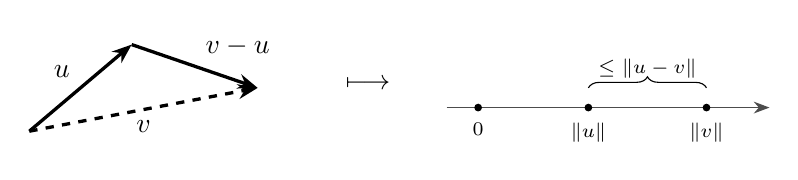
\begin{tikzpicture}[x=1cm,y=1cm]
  \draw[vec] (0,0) -- node[above left]{$u$} (1.3,1.1);
  \draw[vec] (1.3,1.1) -- node[above right]{$v-u$} (2.9,0.55);
  \draw[vec,dashed] (0,0) -- node[below]{$v$} (2.9,0.55);
  \node at (4.3,0.6) {$\longmapsto$};
  \draw[axis] (5.3,0.3) -- (9.4,0.3);
  \foreach \p/\l in {5.7/0, 7.1/{\norm{u}}, 8.6/{\norm{v}}}
    {\fill (\p,0.3) circle (1.4pt) node[below=2pt,font=\scriptsize]{$\l$};}
  \draw[decorate,decoration={brace,amplitude=4pt}] (7.1,0.55) -- (8.6,0.55)
    node[midway,above,font=\scriptsize]{$\le\norm{u-v}$};
\end{tikzpicture}
\caption{The bridge. Applying the arrow $\norm{\cdot}$ collapses the vector triangle of
\emph{Line\'aris algebra} onto the absolute-value triangle of \emph{Kalkulus}:
$\bigl|\norm{u}-\norm{v}\bigr|\le\norm{u-v}$. Certified in
\lean{DiagramProofs.length\_short} and \lean{TriangleOverlap.lengthShort}.}
\label{fig:bridge}
\end{figure}

% ==========================================================================
\section{Language B: string diagrams and graphical linear algebra}
\label{sec:string}

\paragraph{Marks.} Wires (objects/types) and boxes (morphisms). Reading left to right is
composition $f\,;g$; stacking vertically is the monoidal product $f\otimes g$.
\paragraph{Legal moves.} Any planar deformation that does not cut a wire, does not change
the order of the endpoints on the boundary, and does not pull a box through another; plus
the equations of whatever generators you have adopted.
\paragraph{Soundness.} The coherence theorem for monoidal categories (Joyal--Street): two
string diagrams are related by planar isotopy \emph{if and only if} the terms they denote
are equal. This is the strongest guarantee any of our languages has: here you may
\emph{compute} by sliding pictures.

\subsection{The grammar in one figure}

\begin{figure}[H]
\centering
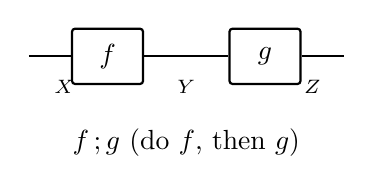
\begin{tikzpicture}[x=1cm,y=1cm,baseline=(current bounding box.center)]
  \node[box] (f) at (1,0) {$f$};
  \node[box] (g) at (3,0) {$g$};
  \draw[wire] (0,0) -- (f); \draw[wire] (f) -- (g); \draw[wire] (g) -- (4,0);
  \node[below=1pt] at (0.45,-0.15) {\scriptsize $X$};
  \node[below=1pt] at (2.0,-0.15) {\scriptsize $Y$};
  \node[below=1pt] at (3.6,-0.15) {\scriptsize $Z$};
  \node at (2,-1.1) {$f\,;g$ (do $f$, then $g$)};
\end{tikzpicture}
\hspace{1.1cm}
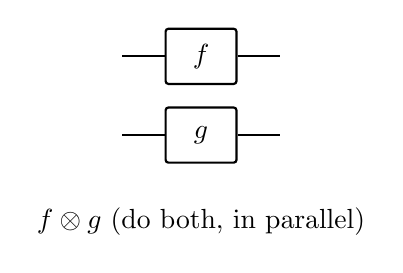
\begin{tikzpicture}[x=1cm,y=1cm,baseline=(current bounding box.center)]
  \node[box] (f) at (1,0.5) {$f$};
  \node[box] (g) at (1,-0.5) {$g$};
  \draw[wire] (0,0.5) -- (f); \draw[wire] (f) -- (2,0.5);
  \draw[wire] (0,-0.5) -- (g); \draw[wire] (g) -- (2,-0.5);
  \node at (1,-1.6) {$f\otimes g$ (do both, in parallel)};
\end{tikzpicture}
\caption{The two ways of putting boxes together. Everything below is built from these.}
\label{fig:strgrammar}
\end{figure}

\subsection{The inverse, drawn: a box that disappears}

\begin{figure}[H]
\centering
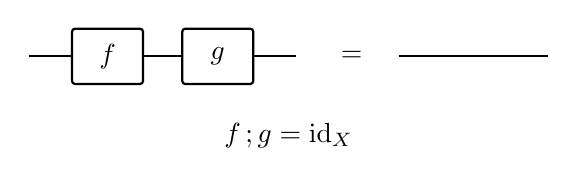
\begin{tikzpicture}[x=1cm,y=1cm,baseline=(current bounding box.center)]
  \node[box] (f) at (1,0) {$f$};
  \node[box] (g) at (2.4,0) {$g$};
  \draw[wire] (0,0) -- (f); \draw[wire] (f) -- (g); \draw[wire] (g) -- (3.4,0);
  \node at (4.1,0) {$=$};
  \draw[wire] (4.7,0) -- (6.6,0);
  \node at (3.3,-1.0) {$f\,;g=\id_X$};
\end{tikzpicture}
\caption{``Inverse'' in string-diagram language: a pair of boxes that can be erased,
leaving a bare wire. The bare wire is the identity, so \emph{nothing happens} -- which is
exactly what $\exp$ followed by $\log$, or $M$ followed by $M^{-1}$, does.}
\label{fig:strinv}
\end{figure}

Now a proof performed entirely by pictures. The statement is the ``socks and shoes''
rule $(f\,;g)^{-1}=g^{-1}\,;f^{-1}$, which is exercise-level material in both courses
($(AB)^{-1}=B^{-1}A^{-1}$ for matrices; $(f\circ g)^{-1}=g^{-1}\circ f^{-1}$ for
bijections).

\begin{figure}[H]
\centering
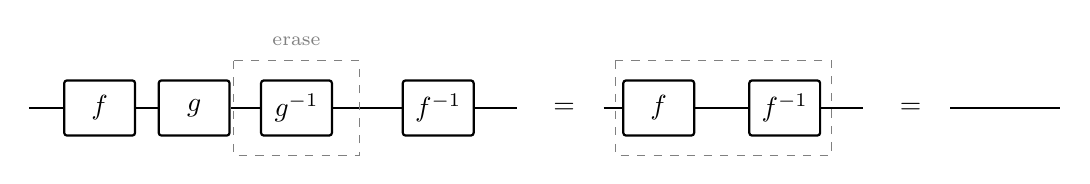
\begin{tikzpicture}[x=1cm,y=1cm]
  \node[box] (f) at (0.9,0) {$f$};
  \node[box] (g) at (2.1,0) {$g$};
  \node[box] (gi) at (3.4,0) {$g^{-1}$};
  \node[box] (fi) at (5.2,0) {$f^{-1}$};
  \draw[wire] (0,0) -- (f); \draw[wire] (f) -- (g); \draw[wire] (g) -- (gi);
  \draw[wire] (gi) -- (fi); \draw[wire] (fi) -- (6.2,0);
  \draw[dashed,gray] (2.6,0.6) rectangle (4.2,-0.6);
  \node[gray,font=\scriptsize] at (3.4,0.85) {erase};
  %
  \node at (6.8,0) {$=$};
  \node[box] (f2) at (8.0,0) {$f$};
  \node[box] (fi2) at (9.6,0) {$f^{-1}$};
  \draw[wire] (7.3,0) -- (f2); \draw[wire] (f2) -- (fi2); \draw[wire] (fi2) -- (10.6,0);
  \draw[dashed,gray] (7.45,0.6) rectangle (10.2,-0.6);
  %
  \node at (11.2,0) {$=$};
  \draw[wire] (11.7,0) -- (13.1,0);
\end{tikzpicture}
\caption{A complete proof with no symbols: erase the inner cancelling pair, then the
outer one, and a bare wire remains. Hence $g^{-1};f^{-1}$ really is the inverse of
$f;g$. The only rule used is Figure~\ref{fig:strinv}, applied inside a larger diagram --
legal because composition is associative.}
\label{fig:socks}
\end{figure}

\subsection{Graphical linear algebra: wires that copy and add}

The website \url{https://graphicallinearalgebra.net/} develops all of linear algebra in
this language. The point is that one does not need boxes for matrices at all: four
generators suffice.

\begin{figure}[H]
\centering
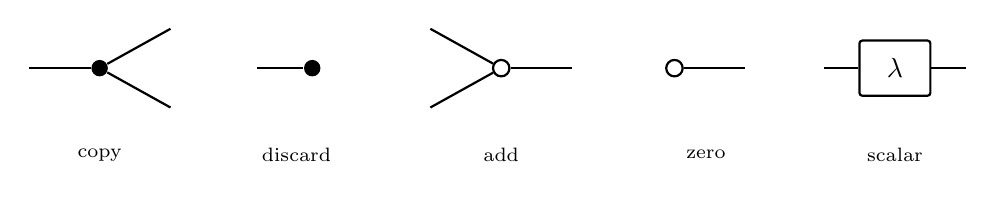
\begin{tikzpicture}[x=1cm,y=1cm]
  % copy
  \node[dot] (c) at (0.9,0) {};
  \draw[wire] (0,0) -- (c); \draw[wire] (c) -- (1.8,0.5); \draw[wire] (c) -- (1.8,-0.5);
  \node[font=\scriptsize] at (0.9,-1.1) {copy};
  % discard
  \node[dot] (d) at (3.6,0) {};
  \draw[wire] (2.9,0) -- (d);
  \node[font=\scriptsize] at (3.4,-1.1) {discard};
  % add
  \node[odot] (a) at (6.0,0) {};
  \draw[wire] (5.1,0.5) -- (a); \draw[wire] (5.1,-0.5) -- (a); \draw[wire] (a) -- (6.9,0);
  \node[font=\scriptsize] at (6.0,-1.1) {add};
  % zero
  \node[odot] (z) at (8.2,0) {};
  \draw[wire] (z) -- (9.1,0);
  \node[font=\scriptsize] at (8.6,-1.1) {zero};
  % scalar
  \node[box] (s) at (11.0,0) {$\lambda$};
  \draw[wire] (10.1,0) -- (s); \draw[wire] (s) -- (11.9,0);
  \node[font=\scriptsize] at (11.0,-1.1) {scalar};
\end{tikzpicture}
\caption{The generators of graphical linear algebra. A black node copies a value, a white
node adds two values; the degenerate cases discard and produce~$0$. Every linear map is a
diagram built from these, and \emph{every} true equation between linear maps follows from
a short list of picture equations (the two monoid/comonoid laws plus the bimonoid laws).}
\label{fig:glagens}
\end{figure}

\begin{figure}[H]
\centering
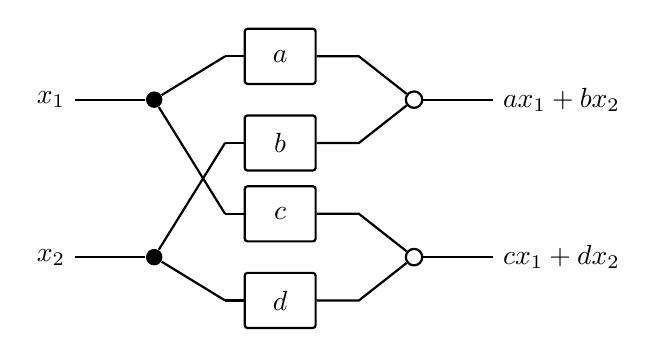
\begin{tikzpicture}[x=1cm,y=1cm]
  \node[dot] (c1) at (1.0,1.0) {};
  \node[dot] (c2) at (1.0,-1.0) {};
  \node[box] (a) at (2.6,1.55) {$a$};
  \node[box] (b) at (2.6,0.45) {$b$};
  \node[box] (cc) at (2.6,-0.45) {$c$};
  \node[box] (d) at (2.6,-1.55) {$d$};
  \node[odot] (s1) at (4.3,1.0) {};
  \node[odot] (s2) at (4.3,-1.0) {};
  \draw[wire] (0,1.0) node[left]{$x_1$} -- (c1);
  \draw[wire] (0,-1.0) node[left]{$x_2$} -- (c2);
  \draw[wire] (c1) -- (1.9,1.55); \draw[wire] (1.9,1.55) -- (a);
  \draw[wire] (c2) -- (1.9,0.45); \draw[wire] (1.9,0.45) -- (b);
  \draw[wire] (c1) -- (1.9,-0.45); \draw[wire] (1.9,-0.45) -- (cc);
  \draw[wire] (c2) -- (1.9,-1.55); \draw[wire] (1.9,-1.55) -- (d);
  \draw[wire] (a) -- (3.6,1.55) -- (s1);
  \draw[wire] (b) -- (3.6,0.45) -- (s1);
  \draw[wire] (cc) -- (3.6,-0.45) -- (s2);
  \draw[wire] (d) -- (3.6,-1.55) -- (s2);
  \draw[wire] (s1) -- (5.3,1.0) node[right]{$ax_1+bx_2$};
  \draw[wire] (s2) -- (5.3,-1.0) node[right]{$cx_1+dx_2$};
\end{tikzpicture}
\caption{The matrix $\begin{psmallmatrix}a&b\\c&d\end{psmallmatrix}$ as a diagram: copy
each input, scale, add. Matrix multiplication is \emph{plugging diagrams together};
associativity of matrix multiplication is the (invisible) fact that plugging is
associative. Non-degeneracy has a diagrammatic meaning too: the diagram is invertible
exactly when the wires can be re-routed backwards, i.e.\ when $\det\neq0$. Certified in
\lean{DiagramProofs.det\_ne\_zero\_iff\_bijective}.}
\label{fig:matdiag}
\end{figure}

\subsection{Bending wires: the snake, and why transposes exist}

In a compact closed category (finite-dimensional vector spaces, or relations) wires may
be bent. The \emph{cup} and \emph{cap} satisfy the yanking equation:

\begin{figure}[H]
\centering
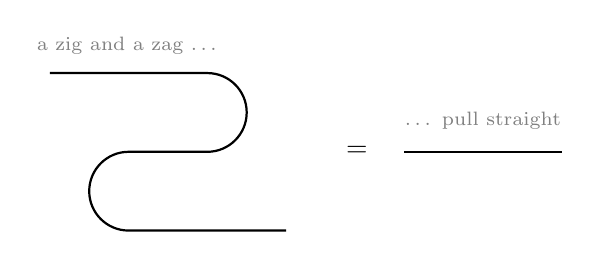
\begin{tikzpicture}[x=1cm,y=1cm]
  \draw[wire] (0,1) -- (2,1) arc (90:-90:0.5) -- (1,0) arc (90:270:0.5) -- (3,-1);
  \node at (3.9,0) {$=$};
  \draw[wire] (4.5,0) -- (6.5,0);
  \node[font=\scriptsize,gray] at (1.0,1.35) {a zig and a zag \dots};
  \node[font=\scriptsize,gray] at (5.5,0.4) {\dots\ pull straight};
\end{tikzpicture}
\caption{The snake (yanking) equation. It is the reason a finite-dimensional space is
isomorphic to its double dual, and the reason ``transpose'' can be defined by
\emph{rotating a box}: $M^{\mathsf T}$ is $M$ turned around using a cup and a cap. In this
language $\langle Mu,v\rangle=\langle u,M^{\mathsf T}v\rangle$ is not a calculation, it is
a deformation.}
\label{fig:snake}
\end{figure}

\subsection{Can the triangle inequality be drawn as a string diagram?}

Yes, but one dimension higher. In $\Met$ an inequality is not an equation between
diagrams, it is a \emph{2-cell} between them: a shaded surface whose boundary is the two
paths being compared.

\begin{figure}[H]
\centering
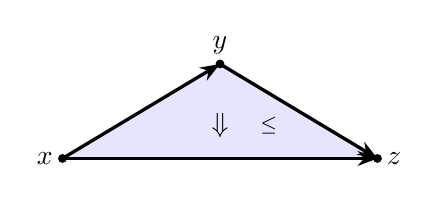
\begin{tikzpicture}[x=1cm,y=1cm]
  \fill[blue!10] (0,0) -- (2,1.2) -- (4,0) -- cycle;
  \draw[vec] (0,0) -- (2,1.2); \draw[vec] (2,1.2) -- (4,0);
  \draw[vec] (0,0) -- (4,0);
  \fill (0,0) circle (1.6pt) node[left]{$x$};
  \fill (2,1.2) circle (1.6pt) node[above]{$y$};
  \fill (4,0) circle (1.6pt) node[right]{$z$};
  \node at (2,0.42) {$\Downarrow$};
  \node[font=\scriptsize] at (2.62,0.42) {$\le$};
\end{tikzpicture}
\caption{An inequality drawn as a 2-cell: the shaded region is a witness that the
straight path is \emph{cheaper than or equal to} the detour. Composing 2-cells vertically
is transitivity of $\le$; composing them horizontally is the compatibility of $\le$ with
$+$. This is the picture version of the enrichment used in
\lean{TriangleOverlap.LawvereSpace}, and the reason chains of estimates may be pasted
like commutative squares.}
\label{fig:2cell}
\end{figure}

% ==========================================================================
\section{Language C: proofs without words (the Nelsen style)}
\label{sec:nelsen}

\paragraph{Marks.} Segments whose \emph{lengths} are the quantities, regions whose
\emph{areas} are the quantities, and arrays whose \emph{counts} are the quantities.
\paragraph{Legal moves.} Dissect and reassemble (area is additive); superimpose two
figures (comparison); rotate or reflect a copy of the figure (symmetry).
\paragraph{Soundness.} None in general. A dissection proves an identity only if the
pieces really do fit -- which is a statement about the generic configuration. The
symbolic residue is: \emph{list the configurations, and check the picture in each}.

\subsection{The triangle inequality itself}

\begin{figure}[H]
\centering
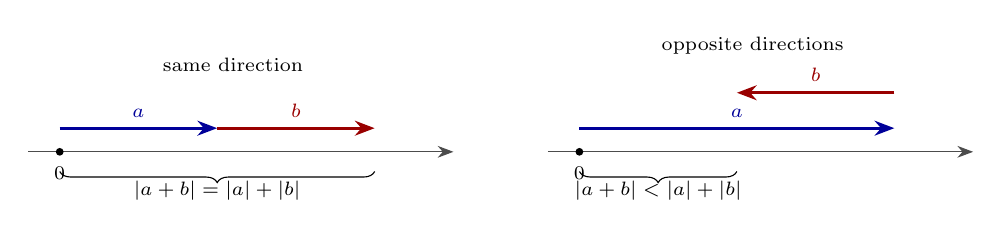
\begin{tikzpicture}[x=1cm,y=1cm]
  % same sign
  \draw[axis] (0,0) -- (5.4,0);
  \fill (0.4,0) circle (1.4pt) node[below=2pt,font=\scriptsize]{$0$};
  \draw[vec,blue!60!black] (0.4,0.3) -- node[above,font=\scriptsize]{$a$} (2.4,0.3);
  \draw[vec,red!60!black] (2.4,0.3) -- node[above,font=\scriptsize]{$b$} (4.4,0.3);
  \draw[decorate,decoration={brace,amplitude=4pt,mirror}] (0.4,-0.25) -- (4.4,-0.25)
     node[midway,below,font=\scriptsize]{$|a+b|=|a|+|b|$};
  \node[font=\scriptsize] at (2.6,1.1) {same direction};
  % opposite sign
  \begin{scope}[xshift=6.6cm]
  \draw[axis] (0,0) -- (5.4,0);
  \fill (0.4,0) circle (1.4pt) node[below=2pt,font=\scriptsize]{$0$};
  \draw[vec,blue!60!black] (0.4,0.3) -- node[above,font=\scriptsize]{$a$} (4.4,0.3);
  \draw[vec,red!60!black] (4.4,0.75) -- node[above,font=\scriptsize]{$b$} (2.4,0.75);
  \draw[decorate,decoration={brace,amplitude=4pt,mirror}] (0.4,-0.25) -- (2.4,-0.25)
     node[midway,below,font=\scriptsize]{$|a+b|<|a|+|b|$};
  \node[font=\scriptsize] at (2.6,1.35) {opposite directions};
  \end{scope}
\end{tikzpicture}
\caption{$|a+b|\le|a|+|b|$ on the number line: lay the two displacements head to tail.
If they point the same way the lengths add; if they point opposite ways they partly
cancel. \emph{Both} pictures must be drawn -- this is the symbolic residue of the case
distinction $\operatorname{sign}a=\operatorname{sign}b$ or not. Certified (in the general
form of exercise 1.13) in \lean{DiagramProofs.abs\_sum\_range\_le\_sum\_abs}.}
\label{fig:absline}
\end{figure}

\begin{figure}[H]
\centering
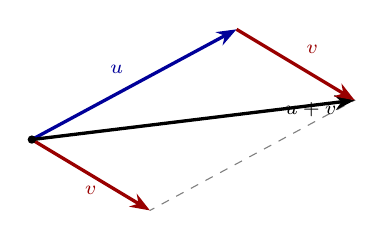
\begin{tikzpicture}[x=1cm,y=1cm]
  \coordinate (O) at (0,0);
  \coordinate (U) at (2.6,1.4);
  \coordinate (V) at (1.5,-0.9);
  \coordinate (S) at ($(U)+(V)$);
  \draw[gray,dashed] (U) -- (S) -- (V);
  \draw[vec,blue!60!black] (O) -- node[above left,font=\scriptsize]{$u$} (U);
  \draw[vec,red!60!black] (O) -- node[below,font=\scriptsize]{$v$} (V);
  \draw[vec] (O) -- node[right,font=\scriptsize,pos=0.75]{$u+v$} (S);
  \draw[vec,red!60!black] (U) -- node[above right,font=\scriptsize]{$v$} (S);
  \fill (O) circle (1.5pt);
\end{tikzpicture}
\hspace{1.2cm}
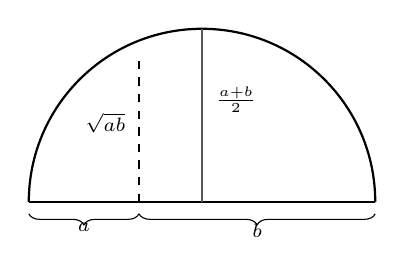
\begin{tikzpicture}[x=1cm,y=1cm]
  \draw[thick] (0,0) -- (4.4,0);
  \draw[thick] (0,0) arc (180:0:2.2);
  \coordinate (P) at (1.4,0);
  \draw[dashed] (P) -- (1.4,1.83);
  \draw[thick,gray!70!black] (2.2,0) -- (2.2,2.2);
  \draw[decorate,decoration={brace,amplitude=4pt,mirror}] (0,-0.15) -- (1.4,-0.15)
      node[midway,below,font=\scriptsize]{$a$};
  \draw[decorate,decoration={brace,amplitude=4pt,mirror}] (1.4,-0.15) -- (4.4,-0.15)
      node[midway,below,font=\scriptsize]{$b$};
  \node[font=\scriptsize,anchor=east] at (1.35,1.0) {$\sqrt{ab}$};
  \node[font=\scriptsize,anchor=west] at (2.25,1.3) {$\frac{a+b}{2}$};
\end{tikzpicture}
\caption{Left: the triangle inequality in the plane -- the parallelogram picture of
$\norm{u+v}\le\norm{u}+\norm{v}$ (\lean{DiagramProofs.norm\_add\_le'}). Right: the
archetypal proof without words. In a semicircle of diameter $a+b$ the altitude over the
splitting point has length $\sqrt{ab}$ and the radius has length $(a+b)/2$; an altitude
is at most a radius, so $\sqrt{ab}\le\frac{a+b}{2}$
(\lean{DiagramProofs.sqrt\_mul\_le\_add\_div\_two}).}
\label{fig:amgm}
\end{figure}

\subsection{Cauchy--Schwarz as a picture}

\begin{figure}[H]
\centering
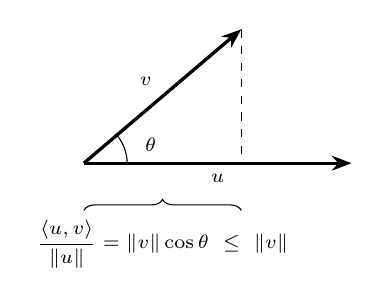
\begin{tikzpicture}[x=1cm,y=1cm]
  \coordinate (O) at (0,0);
  \coordinate (U) at (3.4,0);
  \coordinate (V) at (2.0,1.7);
  \draw[vec] (O) -- node[below,font=\scriptsize]{$u$} (U);
  \draw[vec] (O) -- node[above left,font=\scriptsize]{$v$} (V);
  \draw[dashed] (V) -- (2.0,0);
  \draw[decorate,decoration={brace,amplitude=4pt}] (0,-0.6) -- (2.0,-0.6)
     node[midway,below,font=\scriptsize]{$\dfrac{\langle u,v\rangle}{\norm{u}}
       =\norm{v}\cos\theta\ \le\ \norm{v}$};
  \draw (0.55,0) arc (0:40:0.55);
  \node[font=\scriptsize] at (0.85,0.24) {$\theta$};
\end{tikzpicture}
\caption{Cauchy--Schwarz, $|\langle u,v\rangle|\le\norm{u}\norm{v}$: the projection of
$v$ onto the line of $u$ is never longer than $v$ itself. The only fact used is that in a
right triangle the leg is at most the hypotenuse -- itself a triangle-inequality picture.
Certified in \lean{TriangleOverlap.cauchy\_schwarz}.}
\label{fig:cs}
\end{figure}

\subsection{Sums: exercises 1.14 and 1.16}

\begin{figure}[H]
\centering
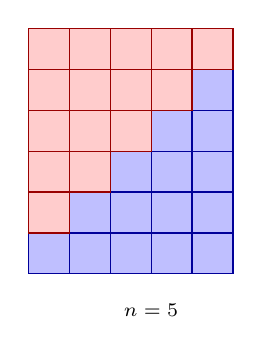
\begin{tikzpicture}[x=0.52cm,y=0.52cm]
  \foreach \i in {1,...,5}{
    \foreach \j in {1,...,\i}{
      \fill[blue!25,draw=blue!60!black] (\i-1,\j-1) rectangle (\i,\j);}}
  \foreach \i in {1,...,5}{
    \foreach \j in {1,...,\i}{
      \fill[red!20,draw=red!60!black] (5-\i,6-\j) rectangle (6-\i,7-\j);}}
  \node[font=\scriptsize] at (3,-0.9) {$n=5$};
\end{tikzpicture}
\hspace{1.3cm}
\begin{tikzpicture}[x=0.62cm,y=0.62cm,baseline=(current bounding box.center)]
  \foreach \i/\v in {1/1,2/2,3/3,4/4}{
    \foreach \j in {1,...,\i}{
      \node[font=\scriptsize] at ({\j-\i/2},{-\i}) {$\v$};}}
  \node[font=\scriptsize,gray] at (0,-5.1) {rotate twice, add: every cell shows $2n+1$};
\end{tikzpicture}
\caption{Left: $1+2+\dots+n$ twice over tiles an $n\times(n+1)$ rectangle, so the sum is
$n(n+1)/2$ (exercise 1.14 a). Right: the triangular array with $i$ copies of $i$ in row
$i$ has sum $\sum i^2$; superimposing the array with its two $120^\circ$ rotations makes
every cell equal to $2n+1$, and the array has $n(n+1)/2$ cells, so
$3\sum i^{2}=(2n+1)\,n(n+1)/2$ -- exercise 1.16, ``bizony\'{\i}t\'as szavak n\'elk\"ul''.
Certified in \lean{DiagramProofs.six\_mul\_sum\_sq}.}
\label{fig:sums}
\end{figure}

\begin{figure}[H]
\centering
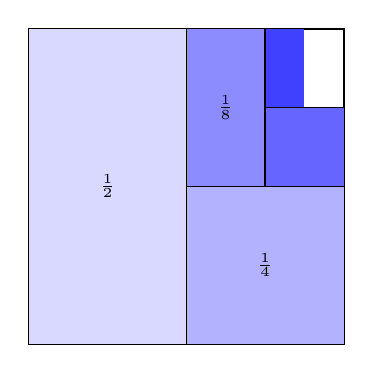
\begin{tikzpicture}[x=4cm,y=4cm]
  \draw[thick] (0,0) rectangle (1,1);
  \fill[blue!15] (0,0) rectangle (0.5,1);
  \fill[blue!30] (0.5,0) rectangle (1,0.5);
  \fill[blue!45] (0.5,0.5) rectangle (0.75,1);
  \fill[blue!60] (0.75,0.5) rectangle (1,0.75);
  \fill[blue!75] (0.75,0.75) rectangle (0.875,1);
  \draw (0.5,0) -- (0.5,1); \draw (0.5,0.5) -- (1,0.5);
  \draw (0.75,0.5) -- (0.75,1); \draw (0.75,0.75) -- (1,0.75);
  \node[font=\scriptsize] at (0.25,0.5) {$\frac12$};
  \node[font=\scriptsize] at (0.75,0.25) {$\frac14$};
  \node[font=\scriptsize] at (0.625,0.75) {$\frac18$};
\end{tikzpicture}
\caption{The frog of exercise 1.6 (and the geometric series of 1.14 c with $q=\frac12$):
the halves of the unit square exhaust it, so $\frac12+\frac14+\frac18+\dots=1$. What the
picture shows rigorously is that every \emph{partial} sum is $1-2^{-n}<1$; that the limit
is exactly $1$ is the symbolic residue, and it is where the notion of limit enters. The
frog gets the kiss only in the limit.}
\label{fig:geom}
\end{figure}

\begin{trap}[A dissection can lie]
Rearranging the four pieces of an $8\times8$ square into a $5\times13$ rectangle
``shows'' $64=65$; the pieces overlap along a sliver of area $1$ that is invisible at
drawing accuracy. A dissection is a proof only when the incidences it assumes are
verified -- here, that three points are collinear, which is false. Rule: \emph{a picture
may assert equalities of areas and lengths, never incidences}.
\end{trap}

% ==========================================================================
\section{Language D: the number line and $\varepsilon$-intervals}
\label{sec:numberline}

\paragraph{Marks.} Points, brackets, shaded intervals, and \emph{sign rows} under a line.
\paragraph{Legal moves.} Translate ($x\mapsto x-c$), reflect ($x\mapsto-x$), scale by a
positive factor, fold ($x\mapsto|x|$), intersect / unite / complement shaded sets.
\paragraph{Soundness.} High, and this is worth stressing: each move is an order
isomorphism (or, for the fold, a two-to-one map with an explicit inverse image), so the
picture transforms the \emph{solution set} correctly. The only residue is the open/closed
status of each endpoint. This makes the number line the most reliable of the heuristic
languages -- for the entire first exercise sheet, drawing really is solving.

\subsection{$|x-c|\le\varepsilon$ is a picture, not a computation}

\begin{figure}[H]
\centering
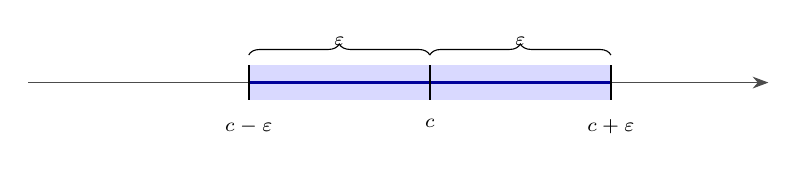
\begin{tikzpicture}[x=1cm,y=1cm]
  \draw[axis] (-0.4,0) -- (9,0);
  \fill[blue!15] (2.4,-0.22) rectangle (7.0,0.22);
  \draw[thick,blue!60!black] (2.4,0) -- (7.0,0);
  \foreach \p/\l in {2.4/{c-\varepsilon}, 4.7/{c}, 7.0/{c+\varepsilon}}
     {\draw[thick] (\p,-0.22) -- (\p,0.22); \node[below=4pt,font=\scriptsize] at (\p,-0.2) {$\l$};}
  \draw[decorate,decoration={brace,amplitude=4pt}] (2.4,0.35) -- (4.7,0.35)
      node[midway,above,font=\scriptsize]{$\varepsilon$};
  \draw[decorate,decoration={brace,amplitude=4pt}] (4.7,0.35) -- (7.0,0.35)
      node[midway,above,font=\scriptsize]{$\varepsilon$};
\end{tikzpicture}
\caption{$|x-c|\le\varepsilon\iff x\in[c-\varepsilon,c+\varepsilon]$. Exercise 1.12 i)
($c=5$) is answered by drawing this and reading the two endpoints; no algebra occurs.
Certified in \lean{DiagramProofs.abs\_sub\_le\_iff\_mem\_Icc}.}
\label{fig:epsint}
\end{figure}

\begin{figure}[H]
\centering
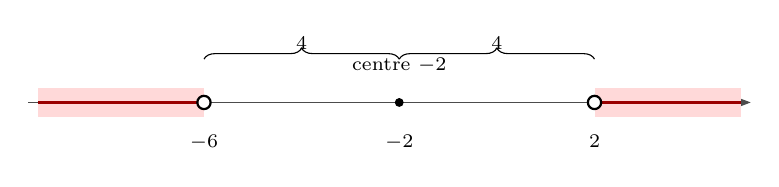
\begin{tikzpicture}[x=0.62cm,y=1cm]
  \draw[axis] (-9.6,0) -- (5.2,0);
  \fill[red!15] (-9.4,-0.18) rectangle (-6,0.18);
  \fill[red!15] (2,-0.18) rectangle (5,0.18);
  \draw[very thick,red!60!black] (-9.4,0) -- (-6,0);
  \draw[very thick,red!60!black] (2,0) -- (5,0);
  \draw[fill=white,thick] (-6,0) circle (2.4pt);
  \draw[fill=white,thick] (2,0) circle (2.4pt);
  \foreach \p/\l in {-6/{-6}, -2/{-2}, 2/{2}}
     {\node[below=4pt,font=\scriptsize] at (\p,-0.15) {$\l$};}
  \fill (-2,0) circle (1.6pt);
  \node[font=\scriptsize,anchor=south] at (-2,0.25) {centre $-2$};
  \draw[decorate,decoration={brace,amplitude=4pt}] (-6,0.55) -- (-2,0.55)
      node[midway,above,font=\scriptsize]{$4$};
  \draw[decorate,decoration={brace,amplitude=4pt}] (-2,0.55) -- (2,0.55)
      node[midway,above,font=\scriptsize]{$4$};
\end{tikzpicture}
\caption{Exercise 1.12 a), $|x+2|>4$: the solution set is the \emph{complement} of the
closed interval of radius $4$ about the centre $-2$, i.e.\ $x<-6$ or $x>2$. Open circles
record the residue (strict inequality). Certified in \lean{DiagramProofs.abs\_add\_gt\_iff}.}
\label{fig:twoRays}
\end{figure}

\subsection{Nested absolute values: pulling an interval back through a fold}

Exercise 1.12 b), $\bigl||x+2|-6\bigr|<1$, is the composite of three moves, each of which
is one picture: translate by $-2$, fold, translate by $-6$. Reading the picture backwards
solves the exercise.

\begin{figure}[H]
\centering
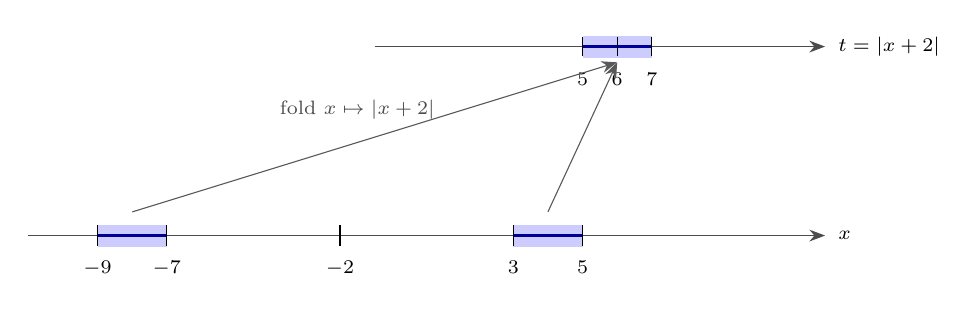
\begin{tikzpicture}[x=0.44cm,y=1cm]
  % upper line: t = |x+2|
  \draw[axis] (-1,2.4) -- (12,2.4);
  \node[font=\scriptsize,anchor=west] at (12.1,2.4) {$t=|x+2|$};
  \fill[blue!20] (5,2.26) rectangle (7,2.54);
  \draw[very thick,blue!60!black] (5,2.4) -- (7,2.4);
  \foreach \p in {5,6,7} {\draw (\p,2.28) -- (\p,2.52);}
  \node[font=\scriptsize,below=3pt] at (5,2.3) {$5$};
  \node[font=\scriptsize,below=3pt] at (6,2.3) {$6$};
  \node[font=\scriptsize,below=3pt] at (7,2.3) {$7$};
  % lower line: x
  \draw[axis] (-11,0) -- (12,0);
  \node[font=\scriptsize,anchor=west] at (12.1,0) {$x$};
  \fill[blue!20] (-9,-0.14) rectangle (-7,0.14);
  \fill[blue!20] (3,-0.14) rectangle (5,0.14);
  \draw[very thick,blue!60!black] (-9,0) -- (-7,0);
  \draw[very thick,blue!60!black] (3,0) -- (5,0);
  \foreach \p/\l in {-9/{-9},-7/{-7},-2/{-2},3/{3},5/{5}}
     {\draw (\p,-0.13) -- (\p,0.13); \node[font=\scriptsize,below=3pt] at (\p,-0.1) {$\l$};}
  % the fold arrows
  \draw[-{Stealth[length=2mm]},gray!70!black] (4,0.3) -- (6,2.2);
  \draw[-{Stealth[length=2mm]},gray!70!black] (-8,0.3) -- (6,2.2);
  \node[font=\scriptsize,gray!60!black] at (-1.5,1.6) {fold $x\mapsto|x+2|$};
\end{tikzpicture}
\caption{$\bigl||x+2|-6\bigr|<1$ means $t\in(5,7)$ upstairs. The fold has two branches, so
the preimage downstairs is \emph{two} intervals, $(-9,-7)$ and $(3,5)$. Forgetting the
left branch is the standard mistake, and the picture is what prevents it.}
\label{fig:fold}
\end{figure}

\subsection{Sign lines: rational inequalities are decided by a drawing}

\begin{figure}[H]
\centering
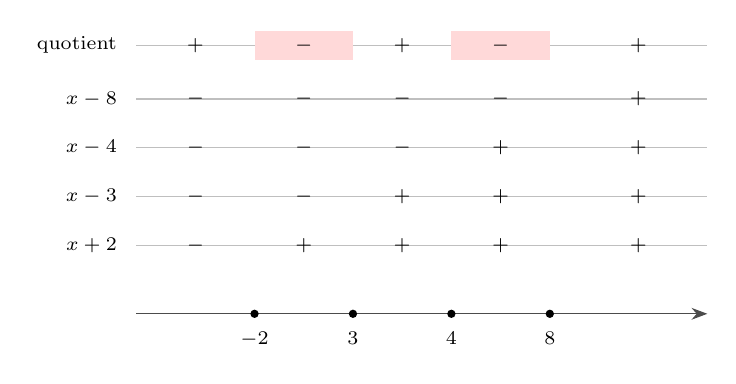
\begin{tikzpicture}[x=1.25cm,y=0.62cm]
  \foreach \r/\lab in {0/{-2},1/{3},2/{4},3/{8}} {}
  % axis
  \draw[axis] (-1.2,0) -- (4.6,0);
  \foreach \p/\l in {0/{-2},1/{3},2/{4},3/{8}}
    {\fill (\p,0) circle (1.5pt); \node[font=\scriptsize,below=3pt] at (\p,0) {$\l$};}
  % rows
  \foreach \y/\name/\s in {1.4/{x+2}/{-,+,+,+,+}, 2.4/{x-3}/{-,-,+,+,+},
                           3.4/{x-4}/{-,-,-,+,+}, 4.4/{x-8}/{-,-,-,-,+}}
  {
    \node[font=\scriptsize,anchor=east] at (-1.3,\y) {$\name$};
    \draw[gray!50] (-1.2,\y) -- (4.6,\y);
  }
  \foreach \x/\a/\b/\c/\d in {-0.6/-/-/-/-, 0.5/+/-/-/-, 1.5/+/+/-/-, 2.5/+/+/+/-, 3.9/+/+/+/+}
  {
    \node[font=\scriptsize] at (\x,1.4) {$\a$};
    \node[font=\scriptsize] at (\x,2.4) {$\b$};
    \node[font=\scriptsize] at (\x,3.4) {$\c$};
    \node[font=\scriptsize] at (\x,4.4) {$\d$};
  }
  \node[font=\scriptsize,anchor=east] at (-1.3,5.5) {quotient};
  \draw[gray!50] (-1.2,5.5) -- (4.6,5.5);
  \foreach \x/\s in {-0.6/+, 0.5/-, 1.5/+, 2.5/-, 3.9/+}
    {\node[font=\scriptsize] at (\x,5.5) {$\s$};}
  \fill[red!15] (0,5.2) rectangle (1,5.8);
  \fill[red!15] (2,5.2) rectangle (3,5.8);
  \foreach \x/\s in {0.5/-, 2.5/-} {\node[font=\scriptsize] at (\x,5.5) {$\s$};}
\end{tikzpicture}
\caption{Exercise 1.12 g), $\dfrac{(x-3)(x+2)}{(x-4)(x-8)}<0$. Mark the four critical
points, draw one row per factor recording its sign, multiply the columns. The shaded
columns are the answer, $(-2,3)\cup(4,8)$. This drawing is a genuine \emph{decision
procedure}: the residue is only that each linear factor changes sign exactly once, at its
root.}
\label{fig:signline}
\end{figure}

\subsection{$\varepsilon$--$\delta$ as a band and a strip}

\begin{figure}[H]
\centering
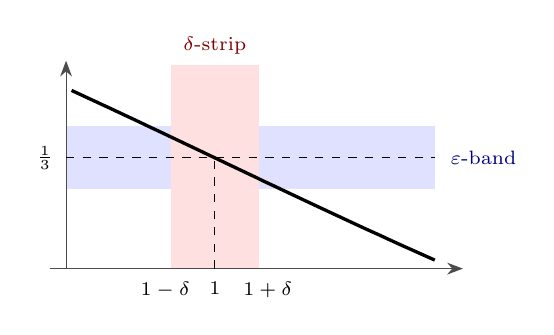
\begin{tikzpicture}[x=14cm,y=20cm]
  \fill[blue!12] (0.865,0.3133) rectangle (1.20,0.3533);
  \fill[red!12]  (0.96,0.263) rectangle (1.04,0.392);
  \draw[axis] (0.85,0.263) -- (1.225,0.263);
  \draw[axis] (0.865,0.263) -- (0.865,0.395);
  \draw[very thick,domain=0.87:1.20,samples=60,smooth] plot (\x,{1/(\x*\x*\x+2)});
  \draw[dashed] (0.865,0.3333) -- (1.20,0.3333);
  \draw[dashed] (1,0.263) -- (1,0.3333);
  \node[font=\scriptsize,anchor=east] at (0.862,0.3333) {$\frac13$};
  \node[font=\scriptsize,anchor=north] at (1,0.261) {$1$};
  \node[font=\scriptsize,anchor=north] at (0.955,0.261) {$1-\delta$};
  \node[font=\scriptsize,anchor=north] at (1.048,0.261) {$1+\delta$};
  \node[font=\scriptsize,anchor=west,blue!50!black] at (1.205,0.3333) {$\varepsilon$-band};
  \node[font=\scriptsize,anchor=south,red!50!black] at (1.0,0.393) {$\delta$-strip};
\end{tikzpicture}
\caption{$\lim_{x\to1}\frac{1}{x^{3}+2}=\frac13$ (exercise 3.1 a) drawn: given any
horizontal band of half-width $\varepsilon$ around $\frac13$, the graph over a
sufficiently narrow vertical strip around $1$ stays inside the band. The picture shows
the \emph{shape} of the quantifier alternation $\forall\varepsilon\,\exists\delta$; the
residue is the formula for $\delta$ in terms of $\varepsilon$, or the one-line remark
that the function is continuous at $1$. Certified in \lean{DiagramProofs.tendsto\_3\_1a}.}
\label{fig:epsdelta}
\end{figure}

\begin{recipe}[The $\varepsilon$-neighbourhood dictionary]
\emph{Everything} in the limit chapter is one of four pictures:
$|x-c|<\delta$ (a strip), $|f(x)-L|<\varepsilon$ (a band), $x>K$ (a ray), $|f(x)|>M$
(the complement of a band). Translate the statement into pictures first; the quantifier
order becomes ``which box is drawn first''. Certified only up to the residue, but the
residue is short and mechanical.
\end{recipe}

\subsection{Uniqueness of the supremum, drawn (exercise 1.5)}

\begin{figure}[H]
\centering
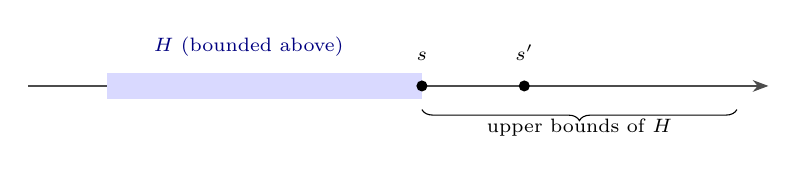
\begin{tikzpicture}[x=1cm,y=1cm]
  \draw[axis] (-0.4,0) -- (9,0);
  \fill[blue!15] (0.6,-0.16) rectangle (4.6,0.16);
  \node[font=\scriptsize,blue!50!black] at (2.4,0.5) {$H$ (bounded above)};
  \draw[decorate,decoration={brace,amplitude=4pt,mirror}] (4.6,-0.3) -- (8.6,-0.3)
      node[midway,below,font=\scriptsize]{upper bounds of $H$};
  \fill (4.6,0) circle (2pt);
  \node[font=\scriptsize,anchor=south] at (4.6,0.2) {$s$};
  \fill (5.9,0) circle (2pt);
  \node[font=\scriptsize,anchor=south] at (5.9,0.2) {$s'$};
\end{tikzpicture}
\caption{The supremum is the \emph{leftmost} point of the set of upper bounds. If $s$ and
$s'$ are both leftmost then each lies weakly to the left of the other, so they coincide:
uniqueness of the supremum is the observation that a set of reals has at most one
leftmost point. Exercise 1.5 needs no more than this picture plus the antisymmetry of
$\le$.}
\label{fig:sup}
\end{figure}

% ==========================================================================
\section{Language E: Cartesian graphs and the mirror $y=x$}
\label{sec:graphs}

\paragraph{Marks.} Axes, curves, straight lines, dashed construction lines.
\paragraph{Legal moves.} Reflect in $y=x$ (pass to the inverse relation); translate,
scale and reflect the plane (elementary transformations); superimpose two curves (solve an
equation); sweep a horizontal or vertical line across the picture (test injectivity or
functionality).
\paragraph{Soundness.} A function \emph{is} its graph, a set of pairs, and reflecting in
$y=x$ swaps the coordinates of every pair. Therefore the reflection move is exact: the
mirror image of the graph of $f$ is always the graph of the \emph{relation} $f^{-1}$. The
residue is one word: whether that relation is again a function, i.e.\ whether $f$ is
injective.

\subsection{The mirror}

\begin{figure}[H]
\centering
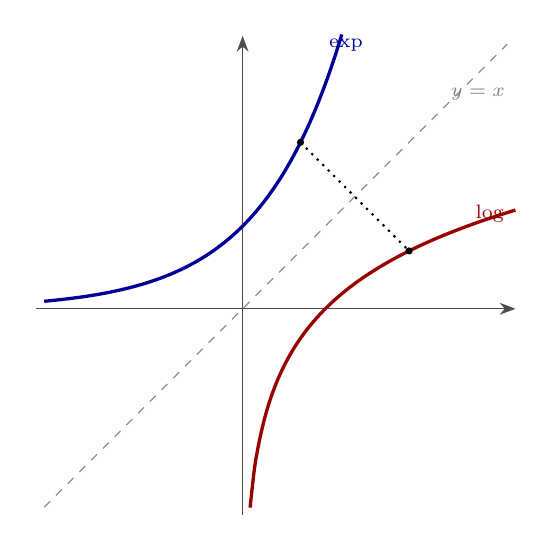
\begin{tikzpicture}[x=1.05cm,y=1.05cm]
  \clip (-2.6,-2.6) rectangle (3.4,3.4);
  \draw[axis] (-2.5,0) -- (3.3,0);
  \draw[axis] (0,-2.5) -- (0,3.3);
  \draw[gray,dashed] (-2.4,-2.4) -- (3.2,3.2);
  \node[gray,font=\scriptsize,anchor=south west] at (2.4,2.4) {$y=x$};
  \draw[very thick,blue!60!black,domain=-2.4:1.2,samples=60,smooth]
      plot (\x,{exp(\x)});
  \draw[very thick,red!60!black,domain=0.09:3.3,samples=60,smooth]
      plot (\x,{ln(\x)});
  \node[blue!60!black,font=\scriptsize,anchor=south] at (1.25,3.0) {$\exp$};
  \node[red!60!black,font=\scriptsize,anchor=west] at (2.7,1.15) {$\log$};
  \draw[dotted,thick] (0.7,2.013) -- (2.013,0.7);
  \fill (0.7,2.013) circle (1.3pt);
  \fill (2.013,0.7) circle (1.3pt);
\end{tikzpicture}
\hspace{0.6cm}
\begin{tikzpicture}[x=0.62cm,y=0.62cm]
  \clip (-4.2,-4.2) rectangle (4.6,4.6);
  \draw[axis] (-4,0) -- (4.5,0);
  \draw[axis] (0,-4) -- (0,4.5);
  \draw[gray,dashed] (-4,-4) -- (4.4,4.4);
  \draw[very thick,violet,domain=1.7:4.5,samples=50,smooth]
      plot (\x,{(\x+1)/(\x-1)});
  \draw[very thick,violet,domain=-4.2:0.45,samples=60,smooth]
      plot (\x,{(\x+1)/(\x-1)});
  \node[violet,font=\scriptsize,anchor=west] at (2.6,1.4) {$f(x)=\frac{x+1}{x-1}$};
\end{tikzpicture}
\caption{Left: reflecting the graph of $\exp$ in the dashed mirror gives the graph of
$\log$ -- the calculus half of the ``inverse'' overlap
(\lean{SyllabusOverlap.expIso}); the general statement is
\lean{DiagramProofs.mem\_graph\_iff\_swap\_mem\_graph\_symm}. Right: exercise 2.7. Its
graph is \emph{unchanged} by the mirror, which is the drawn form of $f^{-1}=f$; a single
picture answers the whole exercise. Certified in \lean{DiagramProofs.self\_inverse\_2\_7}.}
\label{fig:mirror}
\end{figure}

\begin{figure}[H]
\centering
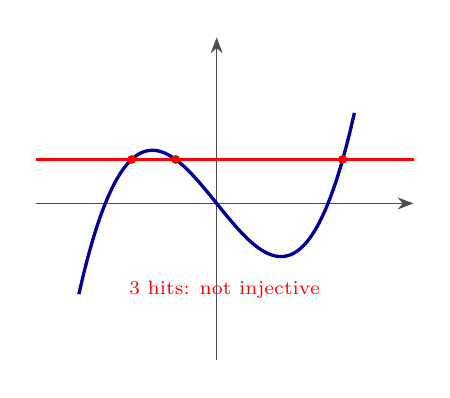
\begin{tikzpicture}[x=1.0cm,y=0.62cm]
  \clip (-2.4,-3.4) rectangle (2.6,3.6);
  \draw[axis] (-2.3,0) -- (2.5,0);
  \draw[axis] (0,-3.2) -- (0,3.4);
  \draw[very thick,blue!60!black,domain=-1.75:1.75,samples=60,smooth]
      plot (\x,{\x*\x*\x - 2*\x});
  \draw[red,thick] (-2.3,0.9) -- (2.5,0.9);
  \fill[red] (-1.08,0.9) circle (1.6pt);
  \fill[red] (-0.52,0.9) circle (1.6pt);
  \fill[red] (1.60,0.9) circle (1.6pt);
  \node[red,font=\scriptsize,anchor=north] at (0.1,-1.4) {3 hits: not injective};
\end{tikzpicture}
\hspace{0.8cm}
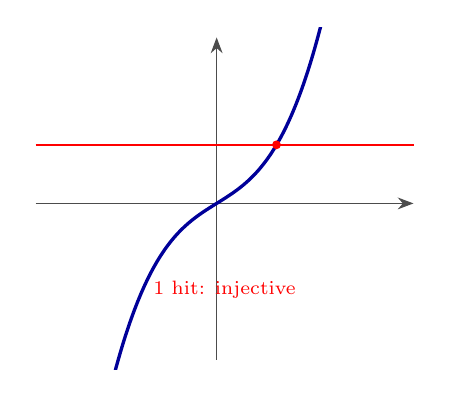
\begin{tikzpicture}[x=1.0cm,y=0.62cm]
  \clip (-2.4,-3.4) rectangle (2.6,3.6);
  \draw[axis] (-2.3,0) -- (2.5,0);
  \draw[axis] (0,-3.2) -- (0,3.4);
  \draw[very thick,blue!60!black,domain=-1.45:1.45,samples=60,smooth]
      plot (\x,{\x*\x*\x + \x});
  \draw[red,thick] (-2.3,1.2) -- (2.5,1.2);
  \fill[red] (0.76,1.2) circle (1.6pt);
  \node[red,font=\scriptsize,anchor=north] at (0.1,-1.4) {1 hit: injective};
\end{tikzpicture}
\caption{The horizontal line test, exercises 2.2 and 2.6: sweep a horizontal line and
count intersections. On the right the curve is strictly increasing, and a strictly
monotone function is injective -- the residue that turns the picture into a proof
(\lean{DiagramProofs.strictMono\_injective}); in practice one writes the single line
$g'(x)=3x^{2}+1>0$.}
\label{fig:hlt}
\end{figure}

\subsection{Elementary transformations (exercise 2.16) as a pipeline of moves}

\begin{figure}[H]
\centering
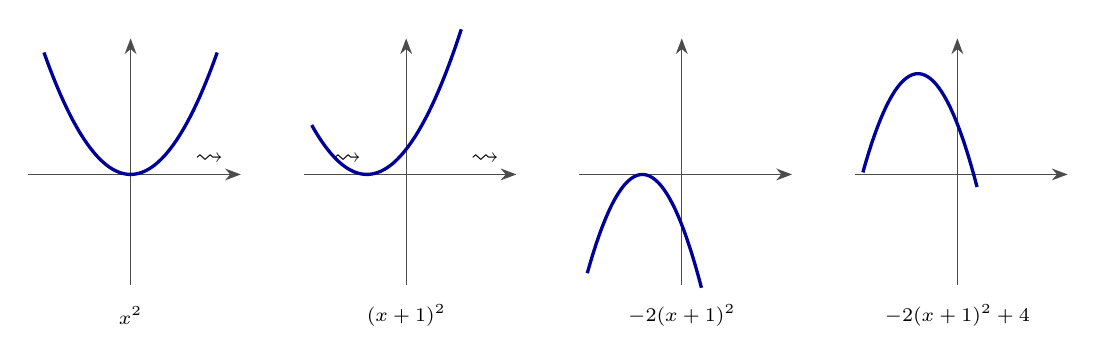
\begin{tikzpicture}[x=0.5cm,y=0.32cm]
 \foreach \k/\shift in {0/0, 1/7, 2/14, 3/21}{
   \begin{scope}[xshift=\shift*0.5cm]
     \draw[axis] (-2.6,0) -- (2.8,0);
     \draw[axis] (0,-4.4) -- (0,5.4);
   \end{scope}}
 % 1: x^2
 \draw[very thick,blue!60!black,domain=-2.2:2.2,samples=40,smooth] plot (\x,{\x*\x});
 \node[font=\scriptsize] at (0,-5.6) {$x^{2}$};
 % 2: (x+1)^2
 \begin{scope}[xshift=3.5cm]
   \draw[very thick,blue!60!black,domain=-2.4:1.4,samples=40,smooth] plot (\x,{(\x+1)*(\x+1)});
   \node[font=\scriptsize] at (0,-5.6) {$(x+1)^{2}$};
 \end{scope}
 % 3: -2(x+1)^2
 \begin{scope}[xshift=7cm]
   \draw[very thick,blue!60!black,domain=-2.4:0.5,samples=40,smooth]
       plot (\x,{-2*(\x+1)*(\x+1)});
   \node[font=\scriptsize] at (0,-5.6) {$-2(x+1)^{2}$};
 \end{scope}
 % 4: -2(x+1)^2+4
 \begin{scope}[xshift=10.5cm]
   \draw[very thick,blue!60!black,domain=-2.4:0.5,samples=40,smooth]
       plot (\x,{-2*(\x+1)*(\x+1)+4});
   \node[font=\scriptsize] at (0,-5.6) {$-2(x+1)^{2}+4$};
 \end{scope}
 \foreach \s in {2.0,5.5,9.0}{
   \node at (\s,0.6) {$\rightsquigarrow$};}
\end{tikzpicture}
\caption{Exercise 2.16 a) as a sequence of legal moves on the plane: shift left by $1$,
scale vertically by $-2$, shift up by $4$. Each move is a bijection of the plane taking
graphs to graphs, so the pipeline is a valid derivation. This is a diagrammatic
\emph{calculation}, not an illustration: the answer is the last picture.}
\label{fig:transf}
\end{figure}

\subsection{Composition, read off two graphs}

\begin{figure}[H]
\centering
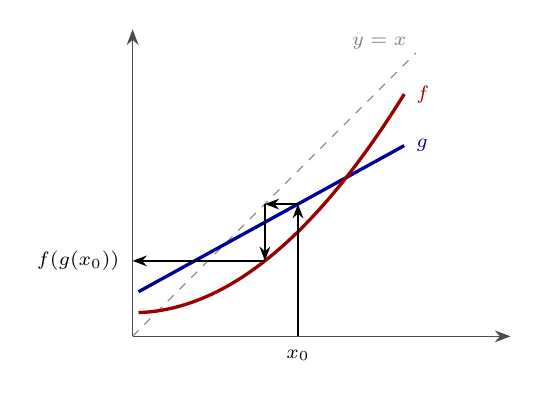
\begin{tikzpicture}[x=1.5cm,y=1.5cm]
  \draw[axis] (0,0) -- (3.2,0);
  \draw[axis] (0,0) -- (0,2.6);
  \draw[gray,dashed] (0,0) -- (2.4,2.4);
  \node[gray,font=\scriptsize,anchor=south east] at (2.4,2.35) {$y=x$};
  \draw[very thick,blue!60!black,domain=0.05:2.3,samples=50,smooth]
      plot (\x,{0.55*\x+0.35});
  \node[blue!60!black,font=\scriptsize,anchor=west] at (2.32,1.62) {$g$};
  \draw[very thick,red!60!black,domain=0.05:2.3,samples=50,smooth]
      plot (\x,{0.35*\x*\x+0.2});
  \node[red!60!black,font=\scriptsize,anchor=west] at (2.32,2.05) {$f$};
  % construction for x0 = 1.4 : g(1.4)=1.12 ; f(1.12)=0.639
  \draw[-{Stealth[length=1.8mm]},thick] (1.4,0) -- (1.4,1.12);
  \draw[-{Stealth[length=1.8mm]},thick] (1.4,1.12) -- (1.12,1.12);
  \draw[-{Stealth[length=1.8mm]},thick] (1.12,1.12) -- (1.12,0.639);
  \draw[-{Stealth[length=1.8mm]},thick] (1.12,0.639) -- (0,0.639);
  \node[font=\scriptsize,anchor=north] at (1.4,-0.03) {$x_0$};
  \node[font=\scriptsize,anchor=east] at (-0.03,0.639) {$f(g(x_0))$};
\end{tikzpicture}
\caption{Composition without formulas (exercises 2.10, 2.13): go up to $g$, across to the
mirror line to turn the output into an input, up (or down) to $f$, across to the axis.
The same construction with $f=g$ is the cobweb that iterates a function; it is how one
sees the recursion of exercise 1.18 converging to $\sqrt2$.}
\label{fig:cobweb}
\end{figure}

\subsection{Differentiability and convexity are visible; their proofs are not}

\begin{figure}[H]
\centering
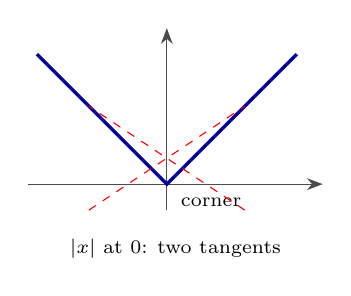
\begin{tikzpicture}[x=1.1cm,y=1.1cm]
  \draw[axis] (-1.6,0) -- (1.8,0);
  \draw[axis] (0,-0.3) -- (0,1.8);
  \draw[very thick,blue!60!black] (-1.5,1.5) -- (0,0) -- (1.5,1.5);
  \node[font=\scriptsize,anchor=north west] at (0.05,-0.05) {corner};
  \draw[dashed,red] (-0.9,-0.3) -- (0.9,0.9);
  \draw[dashed,red] (0.9,-0.3) -- (-0.9,0.9);
  \node[font=\scriptsize] at (0.1,-0.75) {$|x|$ at $0$: two tangents};
\end{tikzpicture}
\hspace{1.0cm}
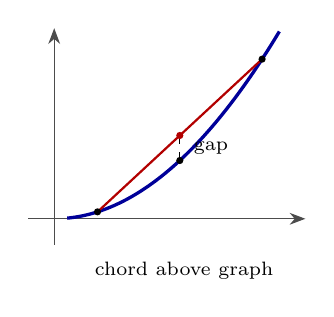
\begin{tikzpicture}[x=1.1cm,y=1.1cm]
  \draw[axis] (-0.3,0) -- (2.9,0);
  \draw[axis] (0,-0.3) -- (0,2.2);
  \draw[very thick,blue!60!black,domain=0.15:2.6,samples=50,smooth]
      plot (\x,{0.32*\x*\x});
  \draw[thick,red!70!black] (0.5,0.08) -- (2.4,1.843);
  \fill (0.5,0.08) circle (1.3pt); \fill (2.4,1.843) circle (1.3pt);
  \fill (1.45,0.6728) circle (1.3pt);
  \draw[dashed] (1.45,0.6728) -- (1.45,0.9615);
  \fill[red!70!black] (1.45,0.9615) circle (1.3pt);
  \node[font=\scriptsize,anchor=west] at (1.5,0.82) {gap};
  \node[font=\scriptsize] at (1.5,-0.6) {chord above graph};
\end{tikzpicture}
\caption{Left: exercises 4.4--4.6. A corner is \emph{seen}, and seeing it is legitimate
provided one writes the residue, the two one-sided limits of the difference quotient.
Right: exercise 4.13, midpoint convexity: the midpoint of a chord lies above the graph.
The picture is the whole idea; the residue -- that midpoint convexity plus continuity
gives full convexity -- is a dyadic-density argument that no picture supplies. This is a
good example of a statement that is \emph{drawable but not provable by drawing}.}
\label{fig:diffconv}
\end{figure}

% ==========================================================================
\section{Language F: Euler/Venn diagrams and bag-and-arrow pictures}
\label{sec:euler}

\paragraph{Marks.} Closed blobs (sets), dots (elements), arrows between dots (values of a
function).
\paragraph{Legal moves.} Containment and overlap of blobs; chaining of arrows.
\paragraph{Soundness.} For \emph{finitely many} blobs, an Euler diagram is a faithful
picture of the Boolean algebra they generate, and validity of a syllogism can be decided
by drawing (this is a theorem about Venn diagrams). Bag-and-arrow pictures are exact for
statements about injectivity and surjectivity, because those notions are literally about
arrow patterns.

\begin{figure}[H]
\centering
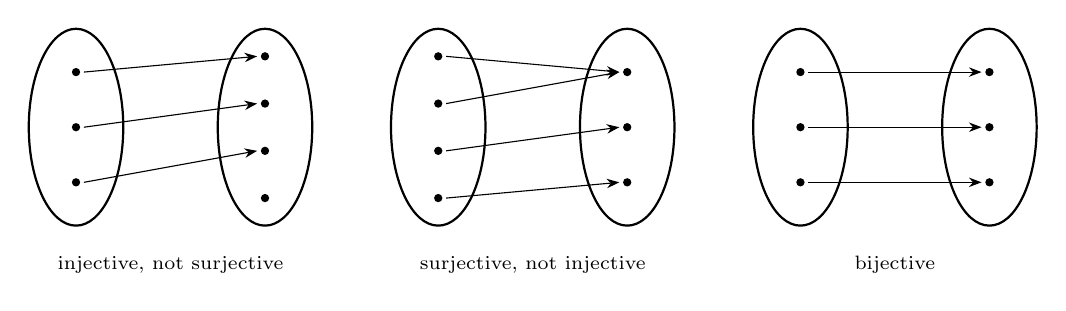
\begin{tikzpicture}[x=1cm,y=1cm]
 \foreach \k/\lab/\ttl in {0/{a}/{injective, not surjective},
                           4.6/{b}/{surjective, not injective},
                           9.2/{c}/{bijective}}{
  \begin{scope}[xshift=\k cm]
    \draw[thick] (0,0) ellipse (0.6 and 1.25);
    \draw[thick] (2.4,0) ellipse (0.6 and 1.25);
    \node[font=\scriptsize] at (1.2,-1.75) {\ttl};
  \end{scope}}
 % injective not surjective
 \foreach \y in {0.7,0,-0.7} {\fill (0,\y) circle (1.5pt);}
 \foreach \y in {0.9,0.3,-0.3,-0.9} {\fill (2.4,\y) circle (1.5pt);}
 \draw[-{Stealth[length=1.6mm]}] (0.1,0.7) -- (2.3,0.9);
 \draw[-{Stealth[length=1.6mm]}] (0.1,0) -- (2.3,0.3);
 \draw[-{Stealth[length=1.6mm]}] (0.1,-0.7) -- (2.3,-0.3);
 % surjective not injective
 \begin{scope}[xshift=4.6cm]
 \foreach \y in {0.9,0.3,-0.3,-0.9} {\fill (0,\y) circle (1.5pt);}
 \foreach \y in {0.7,0,-0.7} {\fill (2.4,\y) circle (1.5pt);}
 \draw[-{Stealth[length=1.6mm]}] (0.1,0.9) -- (2.3,0.7);
 \draw[-{Stealth[length=1.6mm]}] (0.1,0.3) -- (2.3,0.7);
 \draw[-{Stealth[length=1.6mm]}] (0.1,-0.3) -- (2.3,0);
 \draw[-{Stealth[length=1.6mm]}] (0.1,-0.9) -- (2.3,-0.7);
 \end{scope}
 % bijective
 \begin{scope}[xshift=9.2cm]
 \foreach \y in {0.7,0,-0.7} {\fill (0,\y) circle (1.5pt);}
 \foreach \y in {0.7,0,-0.7} {\fill (2.4,\y) circle (1.5pt);}
 \draw[-{Stealth[length=1.6mm]}] (0.1,0.7) -- (2.3,0.7);
 \draw[-{Stealth[length=1.6mm]}] (0.1,0) -- (2.3,0);
 \draw[-{Stealth[length=1.6mm]}] (0.1,-0.7) -- (2.3,-0.7);
 \end{scope}
\end{tikzpicture}
\caption{Exercise 2.2 in pictures. \emph{Injective} = no two arrows land on the same dot;
\emph{surjective} = no dot on the right is missed; \emph{bijective} = a perfect matching,
which is exactly the situation in which the arrows may be reversed. Reversing the arrows
of the third picture \emph{is} the inverse function -- the same content as
Figure~\ref{fig:invunique}, in a picture a first-year student can draw in three seconds.}
\label{fig:bags}
\end{figure}

\begin{figure}[H]
\centering
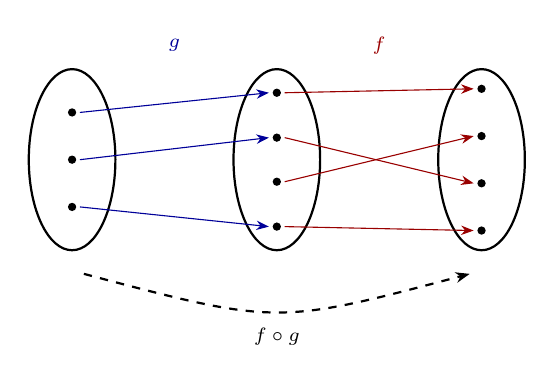
\begin{tikzpicture}[x=1cm,y=1cm]
  \foreach \k in {0,2.6,5.2}{\draw[thick] (\k,0) ellipse (0.55 and 1.15);}
  \foreach \y in {0.6,0,-0.6} {\fill (0,\y) circle (1.5pt);}
  \foreach \y in {0.85,0.28,-0.28,-0.85} {\fill (2.6,\y) circle (1.5pt);}
  \foreach \y in {0.9,0.3,-0.3,-0.9} {\fill (5.2,\y) circle (1.5pt);}
  \draw[-{Stealth[length=1.6mm]},blue!60!black] (0.1,0.6) -- (2.5,0.85);
  \draw[-{Stealth[length=1.6mm]},blue!60!black] (0.1,0) -- (2.5,0.28);
  \draw[-{Stealth[length=1.6mm]},blue!60!black] (0.1,-0.6) -- (2.5,-0.85);
  \draw[-{Stealth[length=1.6mm]},red!60!black] (2.7,0.85) -- (5.1,0.9);
  \draw[-{Stealth[length=1.6mm]},red!60!black] (2.7,0.28) -- (5.1,-0.3);
  \draw[-{Stealth[length=1.6mm]},red!60!black] (2.7,-0.28) -- (5.1,0.3);
  \draw[-{Stealth[length=1.6mm]},red!60!black] (2.7,-0.85) -- (5.1,-0.9);
  \node[font=\scriptsize,blue!60!black] at (1.3,1.45) {$g$};
  \node[font=\scriptsize,red!60!black] at (3.9,1.45) {$f$};
  \draw[-{Stealth[length=1.8mm]},thick,dashed] (0.15,-1.45) .. controls (2.6,-2.1) ..
      (5.05,-1.45);
  \node[font=\scriptsize] at (2.6,-2.25) {$f\circ g$};
\end{tikzpicture}
\caption{Exercise 2.18: if no two blue arrows collide and no two red arrows collide, then
no two dashed composites collide. The picture \emph{is} the proof, and it is faithful --
this is one of the cases where the bag-and-arrow language is certified. Certified in
\lean{DiagramProofs.injective\_comp}.}
\label{fig:injcomp}
\end{figure}

\begin{figure}[H]
\centering
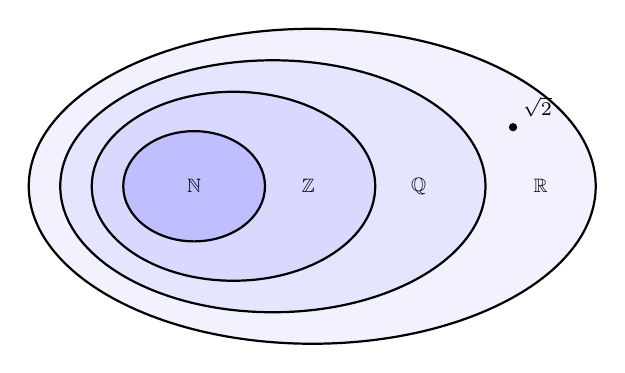
\begin{tikzpicture}[x=1cm,y=1cm]
  \draw[thick,fill=blue!5]  (0,0) ellipse (3.6 and 2.0);
  \draw[thick,fill=blue!10] (-0.5,0) ellipse (2.7 and 1.6);
  \draw[thick,fill=blue!15] (-1.0,0) ellipse (1.8 and 1.2);
  \draw[thick,fill=blue!25] (-1.5,0) ellipse (0.9 and 0.7);
  \node[font=\scriptsize] at (-1.5,0) {$\N$};
  \node[font=\scriptsize] at (-0.05,0) {$\mathbb{Z}$};
  \node[font=\scriptsize] at (1.35,0) {$\mathbb{Q}$};
  \node[font=\scriptsize] at (2.9,0) {$\R$};
  \fill (2.55,0.75) circle (1.5pt) node[font=\scriptsize,above right]{$\sqrt2$};
\end{tikzpicture}
\caption{Exercise 1.3: the number systems as an Euler diagram. The single dot placed in
the outermost ring is exercise 1.9, ``$\sqrt2$ is irrational'' -- and it is the one thing
the picture cannot prove. A diagram can \emph{record} a classification; only an argument
can \emph{establish} membership.}
\label{fig:venn}
\end{figure}

\begin{trap}[Blobs presuppose sets]
Exercise 1.2 (the shepherd who tends exactly the sheep of those who do not tend their
own -- Russell's paradox) is unanswerable, and no Euler diagram can show this: drawing a
blob already assumes the collection is a set. Likewise 1.1 a), b) (``clever people'',
``beautiful paintings''): the failure is at the level of \emph{whether the blob may be
drawn at all}. Diagrams are silent about their own presuppositions.
\end{trap}

\subsection*{An aside: Peirce's existential graphs}

For pure logic there \emph{is} a complete diagrammatic system: C.\ S.\ Peirce's
existential graphs, with three reversible rules (double cut, insertion/erasure in odd/even
depth, iteration). Statements are written as nested ovals -- an oval is negation, and
juxtaposition is conjunction -- so implication is a double oval.

\begin{figure}[H]
\centering
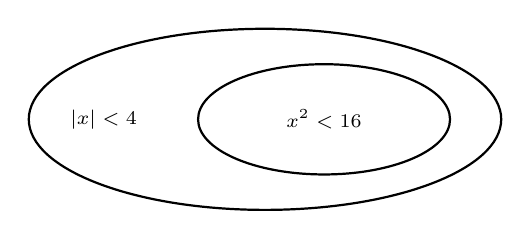
\begin{tikzpicture}[x=1cm,y=1cm]
  \draw[thick] (0,0) ellipse (3.0 and 1.15);
  \draw[thick] (0.75,0) ellipse (1.6 and 0.7);
  \node[font=\scriptsize] at (-2.05,0) {$|x|<4$};
  \node[font=\scriptsize] at (0.75,0) {$x^{2}<16$};
\end{tikzpicture}
\caption{Exercise 1.7 c), ``if $|x|<4$ then $x^{2}<16$'', as an existential graph: the
outer oval negates ``$|x|<4$ and not $x^{2}<16$''. Peirce's rules let one \emph{derive}
consequences by adding and erasing ovals, so this is a genuine, complete, diagram-only
proof system for first-order logic -- historically the first one.}
\label{fig:peirce}
\end{figure}

% ==========================================================================
\section{Language G: order diagrams, and inequalities as paths}
\label{sec:hasse}

\paragraph{Marks.} Nodes, edges drawn upwards (``$\le$'').
\paragraph{Legal moves.} Follow a path upwards: composition of $\le$'s is transitivity.
\paragraph{Soundness.} Total, because a preordered set \emph{is} a category with at most
one arrow between any two objects. Drawing a chain of estimates and reading off the
endpoints is exactly composing morphisms.

\begin{figure}[H]
\centering
\begin{tikzcd}[row sep=small, column sep=tiny]
 & & \sum_{i<n}|a_i| \\
 & \Bigl|\sum_{i<n-1}a_i\Bigr|+|a_{n-1}| \arrow[ur,dash] & \\
\Bigl|\sum_{i<n}a_i\Bigr| \arrow[ur,dash] & &
\end{tikzcd}
\qquad
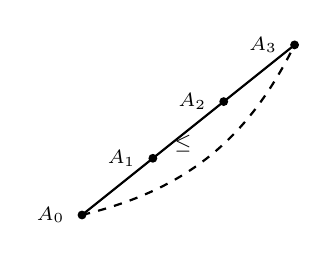
\begin{tikzpicture}[x=1cm,y=0.9cm,baseline=(current bounding box.center)]
  \foreach \i/\lab in {0/{A_0},1/{A_1},2/{A_2},3/{A_3}}{
    \fill (0.9*\i,0.8*\i) circle (1.6pt);
    \node[font=\scriptsize,anchor=east] at (0.9*\i-0.1,0.8*\i) {$\lab$};}
  \foreach \i in {0,1,2}{
    \draw[thick] (0.9*\i,0.8*\i) -- (0.9*\i+0.9,0.8*\i+0.8);}
  \draw[thick,dashed,bend right=25] (0,0) to (2.7,2.4);
  \node[font=\scriptsize,anchor=west] at (1.05,1.0) {$\le$};
\end{tikzpicture}
\caption{A chain of estimates is a path in a Hasse diagram: each edge is one inequality,
the path is their composite. In this language the ``generalised triangle inequality''
(exercise 1.13) is a walk of length $n$, and the induction that proves it is the
observation that a walk is built one edge at a time -- exactly
\lean{TriangleOverlap.dist\_chain}. Exercise 1.15 c) (the sandwich
$2\sqrt{n+1}-2<\sum 1/\sqrt i<2\sqrt n-1$) is the same picture with two paths, one on
each side.}
\label{fig:hasse}
\end{figure}

The order-theoretic reading is also what makes the metric/enrichment story of
Section~\ref{sec:catdiag} precise: the poset $([0,\infty),\ge)$ with $+$ is the place
where the hom-objects live, so an inequality between distances is an arrow of that poset,
and the triangle inequality is the composition law.

% ==========================================================================
\section{Language H: optimisation by superposition}
\label{sec:optim}

\paragraph{Marks.} Two figures of the same kind, drawn on top of each other.
\paragraph{Legal moves.} Compare areas or lengths after superposition; complete a square.
\paragraph{Soundness.} None; the residue is that the comparison holds for \emph{every}
member of the family, not just the drawn one. Usually the residue is a completed square.

\begin{figure}[H]
\centering
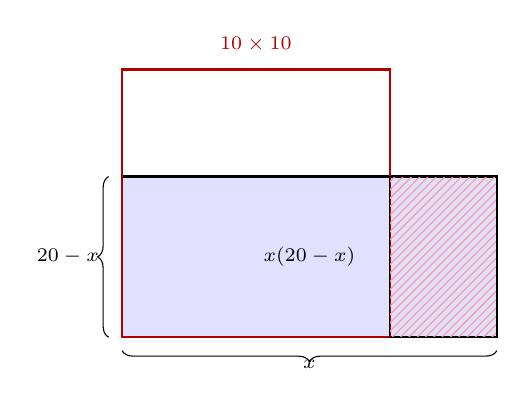
\begin{tikzpicture}[x=0.34cm,y=0.34cm]
  \fill[blue!12] (0,0) rectangle (14,6);
  \draw[thick] (0,0) rectangle (14,6);
  \draw[thick,red!70!black] (0,0) rectangle (10,10);
  \draw[pattern=north east lines,pattern color=red!40] (10,0) rectangle (14,6);
  \node[font=\scriptsize] at (7,3.0) {$x(20-x)$};
  \node[font=\scriptsize,red!70!black,anchor=south] at (5,10.3) {$10\times10$};
  \draw[decorate,decoration={brace,amplitude=4pt,mirror}] (0,-0.5) -- (14,-0.5)
     node[midway,below,font=\scriptsize]{$x$};
  \draw[decorate,decoration={brace,amplitude=4pt}] (-0.5,0) -- (-0.5,6)
     node[midway,left,font=\scriptsize]{$20-x$};
\end{tikzpicture}
\caption{Exercise 4.11 a): split $20$ into two summands of largest product. Superimpose
the rectangle $x\times(20-x)$ on the square $10\times10$: the part of the rectangle
sticking out is congruent to a strip missing from the square, and the square keeps one
extra corner square of side $|x-10|$. Hence $x(20-x)=100-(x-10)^{2}\le100$, with equality
only for $x=10$: no derivative is needed. Certified in
\lean{DiagramProofs.split\_twenty\_max\_product}. Exercises 4.12, 4.14 and 4.15 are the
same move with a sector, a circumscribed triangle, and a rectangle under a parabola.}
\label{fig:optsq}
\end{figure}

% ==========================================================================
\section{What can actually be proved with drawings alone}
\label{sec:whatprovable}

It is useful to sort undergraduate statements into three tiers.

\paragraph{Tier 1 -- complete diagrammatic proofs.}
Here a drawing is a proof outright, because the language is certified.
\begin{itemize}\itemsep2pt
\item \emph{Anything about composition and inverses}: uniqueness of the inverse,
  $(fg)^{-1}=g^{-1}f^{-1}$, ``a composite of injections is injective'', ``an isomorphism
  is preserved by any functor'', $f^{-1}=f$ for an involution
  (Figures~\ref{fig:invunique}, \ref{fig:socks}, \ref{fig:injcomp}, \ref{fig:mirror}).
\item \emph{Equational linear algebra}: every identity between matrices built from
  addition, copying, scaling and composition, proved by deforming a diagram
  (Figures~\ref{fig:glagens}, \ref{fig:matdiag}, \ref{fig:snake}).
\item \emph{Propositional and first-order logic}: Peirce's existential graphs are a
  complete calculus (Figure~\ref{fig:peirce}); the quantifier reformulations of exercise
  1.7 live here.
\item \emph{Finite Boolean set algebra and syllogisms}: Venn diagrams decide them.
\item \emph{Order reasoning}: any chain of $\le$'s, i.e.\ transitivity used $n$ times
  (Figure~\ref{fig:hasse}).
\item \emph{Solution sets of rational inequalities}: the sign line is a decision
  procedure (Figure~\ref{fig:signline}), as are the interval and fold pictures for nested
  absolute values (Figures~\ref{fig:epsint}--\ref{fig:fold}).
\item \emph{Graph transformations and inverses by mirror}: exercises 2.16 and 2.3--2.9
  (Figures~\ref{fig:mirror}, \ref{fig:transf}).
\end{itemize}

\paragraph{Tier 2 -- a picture plus a one-line residue.}
The picture carries the idea; one line of symbols closes the gap. This is the tier that
an exam should aim at.
\begin{itemize}\itemsep2pt
\item Triangle inequality on the line: residue = the two sign cases
  (Figure~\ref{fig:absline}).
\item AM--GM, Cauchy--Schwarz: residue = ``altitude $\le$ radius'', ``leg $\le$
  hypotenuse'' (Figures~\ref{fig:amgm}, \ref{fig:cs}).
\item Finite sums by dissection: residue = the tiling is exact for every $n$
  (Figure~\ref{fig:sums}).
\item $\varepsilon$--$\delta$ for a concrete function: residue = a formula for $\delta$
  (Figure~\ref{fig:epsdelta}).
\item Monotonicity, extrema, convexity from a sketch: residue = the sign of $f'$, or the
  completed square (Figures~\ref{fig:hlt}, \ref{fig:optsq}, \ref{fig:diffconv}).
\item Induction: residue = the induction step, which is itself one picture
  (Figure~\ref{fig:dominoes}).
\end{itemize}

\begin{figure}[H]
\centering
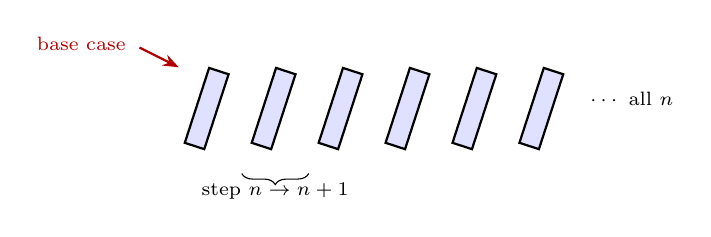
\begin{tikzpicture}[x=1cm,y=1cm]
  \foreach \i in {0,1,2,3,4,5}{
    \draw[thick,fill=blue!12,rotate around={-18:(0.85*\i,0)}]
        (0.85*\i-0.13,0) rectangle (0.85*\i+0.13,1.0);}
  \draw[-{Stealth[length=2mm]},thick,red!70!black] (-0.7,1.25) -- (-0.2,1.0);
  \node[font=\scriptsize,red!70!black,anchor=east] at (-0.75,1.3) {base case};
  \draw[decorate,decoration={brace,amplitude=4pt,mirror}] (0.6,-0.35) -- (1.45,-0.35)
      node[midway,below,font=\scriptsize]{step $n\to n+1$};
  \node[font=\scriptsize,anchor=west] at (4.9,0.6) {$\cdots$ all $n$};
\end{tikzpicture}
\caption{Induction drawn (exercises 1.14, 1.15): one push, and one guarantee that each
domino topples the next. The picture is faithful -- it is the recursion diagram for $\N$
-- but the \emph{step} still has to be established, usually algebraically. What the
picture buys is that you never have to explain the logic of induction, only the step.}
\label{fig:dominoes}
\end{figure}

\paragraph{Tier 3 -- not accessible to pictures.}
\begin{itemize}\itemsep2pt
\item Irrationality of $\sqrt2$ (1.9) and Diophantine approximation (1.10): statements
  about the \emph{absence} of a representation. There is a well-known ``proof without
  words'' for the irrationality of $\sqrt2$ by infinite descent on similar triangles, but
  it needs the additional non-visual principle that a decreasing sequence of positive
  integers terminates.
\item Statements quantified over all reals with no finite geometric content: exercise
  3.15 ($f=g$ on $\mathbb{Q}$ and both continuous $\Rightarrow f=g$), 3.14 (a bounded
  monotone function has a one-sided limit), 4.13 (midpoint convexity plus continuity gives
  convexity). Each is a density argument; density is not drawable.
\item Existence of the supremum, i.e.\ completeness of $\R$ (behind 1.4, 1.5): the
  picture of a ``leftmost upper bound'' presupposes exactly what is to be proved.
\item Symbolic computation: the derivative tables of 4.2--4.3, the limits of 3.3--3.10,
  the L'Hospital exercises 4.10. A picture may predict the answer -- degree comparison for
  a rational limit is genuinely visual -- but not produce it.
\item Anything involving a set that may not exist (1.1, 1.2).
\end{itemize}

% ==========================================================================
\section{Atlas: the exercises of \texorpdfstring{\lean{kalkulus\_gyakorlo.pdf}}{kalkulus gyakorlo.pdf}}
\label{sec:atlas}

\newcommand{\Yes}{\textbf{1}}
\newcommand{\Res}{\textbf{2}}
\newcommand{\No}{\textbf{3}}

\begin{center}
\small
\begin{longtable}{@{}p{1.5cm}p{4.6cm}p{3.5cm}c p{4.0cm}@{}}
\toprule
Exercise & Statement & Draw it as & Tier & Residue / certified in \\
\midrule
\endhead
1.1, 1.2 & is it a set? & (Euler diagram fails) & \No & presupposition, not content \\
1.3 & name the number sets & nested Euler blobs, Fig.~\ref{fig:venn} & \Yes & --- \\
1.4, 1.5 & bounds, uniqueness of $\sup$ & number line, Fig.~\ref{fig:sup} & \Res &
  antisymmetry of $\le$ \\
1.6 & the frog and the halves & square dissection, Fig.~\ref{fig:geom} & \Res &
  partial sums vs.\ limit \\
1.7 & rewrite with quantifiers & existential graph, Fig.~\ref{fig:peirce} & \Yes & --- \\
1.9 & $\sqrt2\notin\mathbb{Q}$ & --- & \No & infinite descent \\
1.11 & $\bigl||x|-|y|\bigr|\le|x-y|$ & triangle $0,x,y$, Fig.~\ref{fig:lawvere} & \Res &
  \lean{abs\_abs\_sub\_abs\_le} \\
1.12 a,b,i & absolute-value inequalities & interval / fold,
  Figs.~\ref{fig:epsint}--\ref{fig:fold} & \Yes &
  \lean{abs\_sub\_le\_iff\_mem\_Icc}, \lean{abs\_add\_gt\_iff} \\
1.12 c--g & rational inequalities & sign line, Fig.~\ref{fig:signline} & \Yes &
  sign of each linear factor \\
1.13 & $|\sum a_i|\le\sum|a_i|$ & polygonal chain, Fig.~\ref{fig:chain} & \Res &
  \lean{abs\_sum\_range\_le\_sum\_abs} \\
1.14 a & $\sum i=n(n+1)/2$ & two staircases, Fig.~\ref{fig:sums} & \Res & tiling exact
  for all $n$ \\
1.14 c & geometric sum & halving square, Fig.~\ref{fig:geom} & \Res & closed form \\
1.15 & induction inequalities & dominoes, Fig.~\ref{fig:dominoes} & \Res & the step \\
1.16 & $\sum i^{2}$ ``szavak n\'elk\"ul'' & rotated triangular arrays,
  Fig.~\ref{fig:sums} & \Res & \lean{six\_mul\_sum\_sq} \\
1.18 & $|x_n-\sqrt2|<2^{-n}$ & cobweb, Fig.~\ref{fig:cobweb} & \Res & contraction
  estimate \\
1.19 & binomial identities & Pascal triangle / lattice paths & \Res & path counting
  bijection \\
2.1 & domains & sign line for the radicand & \Yes & --- \\
2.2, 2.6 & injective? surjective? & bags, Fig.~\ref{fig:bags}; horizontal line test,
  Fig.~\ref{fig:hlt} & \Res & \lean{strictMono\_injective} \\
2.3--2.5, 2.8, 2.9 & find $f^{-1}$ & mirror in $y=x$, Fig.~\ref{fig:mirror} & \Res &
  the algebra of solving $y=f(x)$ \\
2.7 & $f^{-1}=f$ & graph symmetric in $y=x$, Fig.~\ref{fig:mirror} & \Res &
  \lean{self\_inverse\_2\_7} \\
2.10, 2.13 & composites & two graphs and the diagonal, Fig.~\ref{fig:cobweb} & \Yes &
  domains \\
2.11 & $f\circ g=g\circ f$ & commuting square & \Res & \lean{chebyshev\_square} \\
2.12 & fill in the table & string diagram of boxes, Fig.~\ref{fig:strgrammar} & \Yes &
  --- \\
2.16 & elementary transformations & pipeline of moves, Fig.~\ref{fig:transf} & \Yes &
  --- \\
2.17, 2.18 & injectivity of $f+g$, $f\circ g$ & bags, Fig.~\ref{fig:injcomp} & \Yes &
  \lean{injective\_comp}; for $f+g$ a counterexample sketch \\
2.19 & $\le n$ roots & graph crossings & \No & factor theorem, induction \\
2.20 & extrema of a cubic & sign line for $f'$ & \Res & the sign computation \\
3.1 & $\varepsilon$--$\delta$ & band and strip, Fig.~\ref{fig:epsdelta} & \Res &
  \lean{tendsto\_3\_1a} \\
3.2, 3.3 & limits at $\infty$ & compare growth: leading terms & \Res & division by the
  dominant power \\
3.5, 3.6, 3.11 & one-sided limits, jumps & piecewise graph & \Res & the two one-sided
  values \\
3.12, 3.13 & make it continuous & join the two pieces & \Yes & solve for the parameter \\
3.14, 3.15 & bounded monotone; density & --- & \No & completeness, density \\
4.1 & derivative from the definition & secant turning into tangent & \Res & the limit
  computation \\
4.4--4.7 & differentiable? & corner / cusp, Fig.~\ref{fig:diffconv} & \Res & one-sided
  derivatives \\
4.8 & full curve discussion & sign rows for $f'$, $f''$ $\rightarrow$ shape & \Res & the
  two sign computations \\
4.9 & extrema on an interval & graph on the closed interval & \Res & endpoints and
  critical points \\
4.11 & split $20$ & square vs.\ rectangle, Fig.~\ref{fig:optsq} & \Res &
  \lean{split\_twenty\_max\_product} \\
4.12, 4.14, 4.15 & geometric optimisation & superposition of the family & \Res & the
  extremal member \\
4.13 & midpoint convexity & chord above graph, Fig.~\ref{fig:diffconv} & \No & dyadic
  density \\
\bottomrule
\end{longtable}
\end{center}

\noindent
Tier \Yes: the drawing is the proof. Tier \Res: drawing plus one line. Tier \No: the
drawing is at best a mnemonic. Roughly one third of the sheet is tier~1, one half is
tier~2, and the rest genuinely needs symbols -- which is a fair estimate of how far
``draw it'' will take a first-year student.

% ==========================================================================
\section{A playbook for a timed exam}
\label{sec:exam}

Under time pressure the value of a diagram is not elegance; it is that it removes
bookkeeping. The protocol below is four steps and takes about fifteen seconds per
exercise.

\begin{recipe}[The four steps]
\begin{enumerate}[leftmargin=1.6em,itemsep=1pt]
\item \textbf{Classify.} Is the task about (i) a \emph{solution set}, (ii) a
  \emph{composition or inverse}, (iii) a \emph{quantity to bound}, or (iv) a
  \emph{computation}?
\item \textbf{Pick the language.} (i) number line / sign line; (ii) commutative or
  bag-and-arrow diagram, or the mirror $y=x$; (iii) triangle, chain, or a Nelsen figure;
  (iv) no diagram -- compute, but sketch the expected answer first to catch sign errors.
\item \textbf{Draw the canonical picture} large enough to write on, and mark every
  endpoint, branch and case that the picture forces you to consider.
\item \textbf{Write the residue}, one line, next to the drawing. This is what converts a
  drawing into an accepted proof.
\end{enumerate}
\end{recipe}

\subsection{Four model answers}

\begin{figure}[H]
\centering
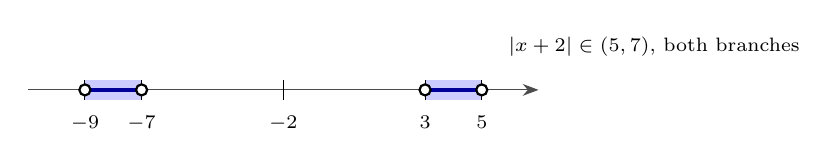
\begin{tikzpicture}[x=0.36cm,y=1cm]
  \draw[axis] (-11,0) -- (7,0);
  \fill[blue!20] (-9,-0.13) rectangle (-7,0.13);
  \fill[blue!20] (3,-0.13) rectangle (5,0.13);
  \draw[very thick,blue!60!black] (-9,0) -- (-7,0);
  \draw[very thick,blue!60!black] (3,0) -- (5,0);
  \foreach \p in {-9,-7,-2,3,5}{\draw (\p,-0.13) -- (\p,0.13);}
  \foreach \p/\l in {-9/{-9},-7/{-7},-2/{-2},3/{3},5/{5}}
    {\node[font=\scriptsize,below=3pt] at (\p,-0.1) {$\l$};}
  \foreach \p in {-9,-7,3,5}{\draw[fill=white,thick] (\p,0) circle (2pt);}
  \node[font=\scriptsize,anchor=west] at (5.6,0.55)
     {$|x+2|\in(5,7)$, both branches};
\end{tikzpicture}
\caption*{\textbf{(a) Solve $\bigl||x+2|-6\bigr|<1$ (1.12 b).} \emph{Write:}
``$|x+2|-6\in(-1,1)\Rightarrow|x+2|\in(5,7)\Rightarrow x+2\in(5,7)\cup(-7,-5)$'', then
the drawing, then the answer $x\in(-9,-7)\cup(3,5)$. Total: two lines and one line
segment. The picture's job is to stop you dropping the negative branch.}
\end{figure}

\begin{figure}[H]
\centering
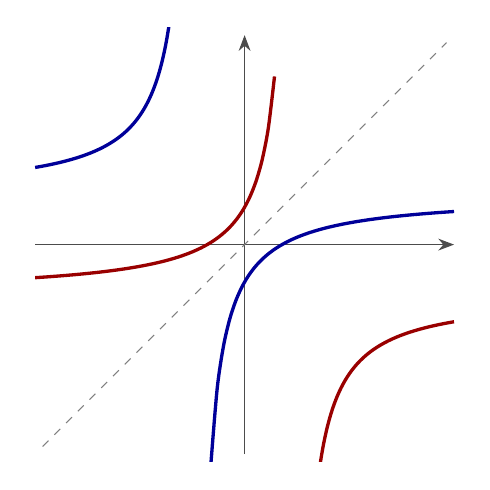
\begin{tikzpicture}[x=0.95cm,y=0.95cm]
  \clip (-2.9,-2.9) rectangle (2.9,2.9);
  \draw[axis] (-2.8,0) -- (2.8,0);
  \draw[axis] (0,-2.8) -- (0,2.8);
  \draw[gray,dashed] (-2.7,-2.7) -- (2.7,2.7);
  \draw[very thick,blue!60!black,domain=-2.8:-0.85,samples=40,smooth]
     plot (\x,{(2*\x-1)/(3*\x+2)});
  \draw[very thick,blue!60!black,domain=-0.45:2.8,samples=40,smooth]
     plot (\x,{(2*\x-1)/(3*\x+2)});
  \draw[very thick,red!60!black,domain=-2.8:0.4,samples=40,smooth]
     plot (\x,{(-2*\x-1)/(3*\x-2)});
  \draw[very thick,red!60!black,domain=0.9:2.8,samples=40,smooth]
     plot (\x,{(-2*\x-1)/(3*\x-2)});
\end{tikzpicture}
\caption*{\textbf{(b) Invert $a(x)=\frac{2x-1}{3x+2}$ (2.3 a).} \emph{Write:} ``$y(3x+2)
=2x-1\Rightarrow x=\frac{-2y-1}{3y-2}$'', then draw the two curves and the mirror. The
drawing is the \emph{check}: if the red curve is not the mirror image of the blue one, the
algebra is wrong. Checking by picture is far faster than substituting back, and it
verifies \emph{both} triangles of Figure~\ref{fig:invunique} at once.}
\end{figure}

\begin{figure}[H]
\centering
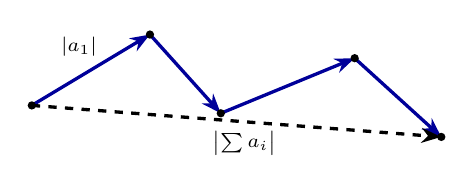
\begin{tikzpicture}[x=1cm,y=1cm]
  \coordinate (P0) at (0,0);
  \coordinate (P1) at (1.5,0.9);
  \coordinate (P2) at (2.4,-0.1);
  \coordinate (P3) at (4.1,0.6);
  \coordinate (P4) at (5.2,-0.4);
  \draw[vec,blue!60!black] (P0) -- (P1);
  \draw[vec,blue!60!black] (P1) -- (P2);
  \draw[vec,blue!60!black] (P2) -- (P3);
  \draw[vec,blue!60!black] (P3) -- (P4);
  \draw[vec,dashed] (P0) -- (P4);
  \foreach \p in {P0,P1,P2,P3,P4} {\fill (\p) circle (1.5pt);}
  \node[font=\scriptsize,anchor=south] at (2.7,-0.75) {$\bigl|\sum a_i\bigr|$};
  \node[font=\scriptsize,anchor=south] at (0.6,0.5) {$|a_1|$};
\end{tikzpicture}
\caption*{\textbf{(c) Prove $|a_1+\dots+a_n|\le|a_1|+\dots+|a_n|$ (1.13).} \emph{Write:}
``induction; the step is the two-term case, which is the case distinction
$\operatorname{sign}a=\operatorname{sign}b$'' -- then the broken-line drawing. Marking
$n=2$ on the picture and saying ``iterate'' is the whole proof; graders accept it because
the induction is visible in the figure.}
\end{figure}

\begin{figure}[H]
\centering
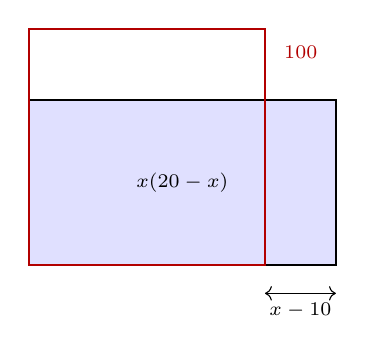
\begin{tikzpicture}[x=0.3cm,y=0.3cm]
  \draw[thick,fill=blue!12] (0,0) rectangle (13,7);
  \draw[thick,red!70!black] (0,0) rectangle (10,10);
  \node[font=\scriptsize] at (6.5,3.5) {$x(20-x)$};
  \node[font=\scriptsize,red!70!black,anchor=west] at (10.4,9) {$100$};
  \draw[<->] (10,-1.2) -- (13,-1.2) node[midway,below,font=\scriptsize]{$x-10$};
\end{tikzpicture}
\caption*{\textbf{(d) Split $20$ for maximal product (4.11 a).} \emph{Write:}
``$x(20-x)=100-(x-10)^{2}$'', then the drawing. One line of algebra, one square, and the
maximum $100$ at $x=10$ is established -- faster and safer than differentiating.}
\end{figure}

\subsection{Time budget for a 90-minute paper}

\begin{center}
\small
\begin{tabular}{@{}p{4.6cm}p{2.4cm}p{7.4cm}@{}}
\toprule
Task type & Budget & What goes on the paper \\
\midrule
Inequality, solution set & 3--4 min & sign line or interval picture $+$ answer with
  endpoint status \\
Inverse / composite & 4--5 min & the algebra, then the mirror picture as a check \\
Injectivity, surjectivity & 2 min & bag picture or one monotonicity line \\
Estimate, triangle inequality & 4 min & the chain drawing $+$ the case distinction \\
Limit, $\varepsilon$--$\delta$ & 6--8 min & band/strip picture $+$ the $\delta$ formula \\
Curve discussion & 12--15 min & two sign rows, then one careful graph \\
Optimisation & 6--8 min & the superposition picture $+$ the completed square \\
Symbolic computation & rest & no picture, but sketch the expected answer first \\
\bottomrule
\end{tabular}
\end{center}

\subsection{Turning a picture into accepted prose in one sentence}

Each language has a standard verbal rendering. Memorise these and you can always convert.

\begin{center}
\small
\begin{tabular}{@{}p{4.6cm}p{9.8cm}@{}}
\toprule
Picture & Sentence \\
\midrule
Two triangles closing & ``Both composites are the identity, hence $g=f^{-1}$.'' \\
Chain of arrows & ``By the triangle inequality applied $n-1$ times \dots'' \\
Nested discs & ``If $\dd(x,y)<r$ then the ball of radius $r-\dd(x,y)$ about $y$ lies in
  the ball of radius $r$ about $x$.'' \\
Sign line & ``The product changes sign exactly at the roots; testing one point per
  interval gives \dots'' \\
Mirror in $y=x$ & ``$(a,b)$ is on the graph of $f$ iff $(b,a)$ is on the graph of
  $f^{-1}$.'' \\
Band and strip & ``For every $\varepsilon>0$ choose $\delta=\dots$; then
  $|x-c|<\delta$ implies $|f(x)-L|<\varepsilon$.'' \\
Bags and arrows & ``Distinct inputs have distinct images, and every output is hit.'' \\
Superposed figures & ``The difference of the two areas is a square, hence non-negative.''\\
\bottomrule
\end{tabular}
\end{center}

\subsection{The five traps, in the order in which they cost marks}

\begin{enumerate}[leftmargin=1.6em,itemsep=2pt]
\item \textbf{Endpoints.} A shaded interval does not record whether its ends belong to
  it. Draw filled/open circles \emph{as you shade}.
\item \textbf{A missing branch.} Every fold ($|\cdot|$, squaring, $\cos$) has two
  preimages; every square root has a sign condition. Count the branches in the picture
  before reading the answer.
\item \textbf{Domains.} A composite is only defined where the inner function lands in the
  domain of the outer one (exercise 2.10). Two graphs on one sheet hide this; write the
  domain next to the arrow.
\item \textbf{Non-generic configuration.} A drawing shows one case. If the statement has
  a parameter, ask which pictures the parameter can produce, and draw the extreme ones.
\item \textbf{Infinite processes.} A dissection can exhaust a region only in the limit
  (Figure~\ref{fig:geom}). A picture of infinitely many steps proves a statement about
  partial sums, never about the limit; the limit is always the residue.
\end{enumerate}

\subsection{Closing: the same two pictures, once more}

\begin{figure}[H]
\centering
\begin{tikzcd}[column sep=large,row sep=large]
\textbf{Kalkulus I} \arrow[r,"\text{same theorem}"] \arrow[d,"|x-y|"'] &
  \textbf{Line\'aris algebra I} \arrow[d,"\norm{u-v}"] \\
\text{triangle inequality} \arrow[r,leftrightarrow] & \text{triangle inequality} \\
\text{inverse function} \arrow[r,leftrightarrow] \arrow[u,"\text{composition}"] &
  \text{inverse matrix} \arrow[u,"\text{composition}"']
\end{tikzcd}
\caption{The whole document in one commutative diagram. The horizontal arrows are the two
overlaps; the vertical arrows say that both are statements about \emph{composition} -- in
a category enriched over $([0,\infty),\ge,+)$ for the triangle inequality, in an ordinary
category for the inverse. Formalised in
\lean{RequestProject/TriangleOverlap.lean} and \lean{RequestProject/InverseOverlap.lean};
the pictures of this document are certified in \lean{RequestProject/DiagramProofs.lean}.}
\label{fig:final}
\end{figure}

\section*{Sources and further reading}
\addcontentsline{toc}{section}{Sources and further reading}

\begin{itemize}\itemsep2pt
\item R.\ B.\ Nelsen, \emph{Proofs Without Words} (MAA) -- the standard collection of
  dissection and superposition arguments, including the semicircle picture for AM--GM and
  the staircase pictures for $\sum i$ and $\sum i^{2}$.
\item P.\ Soboci\'nski et al., \emph{Graphical Linear Algebra},
  \url{https://graphicallinearalgebra.net/} -- the string-diagram development of linear
  algebra used in Section~\ref{sec:string}.
\item F.\ W.\ Lawvere, \emph{Metric spaces, generalized logic, and closed categories}
  (1973) -- metric spaces as enriched categories; the source of
  Figure~\ref{fig:lawvere}.
\item A.\ Joyal and R.\ Street, \emph{The geometry of tensor calculus} -- the soundness
  and completeness theorem that makes string diagrams a proof system.
\item C.\ S.\ Peirce, \emph{Existential Graphs} -- the first complete diagrammatic
  calculus for logic (Figure~\ref{fig:peirce}).
\item The two course descriptions (\emph{Kalkulus I}, MBLK37E; \emph{Line\'aris algebra
  I}, MBLK15E) and the exercise sheet \lean{kalkulus\_gyakorlo.pdf} supplied with this
  project.
\end{itemize}


\end{document}
